\documentclass[UTF8]{article} 
\usepackage{graphicx}
\usepackage{subfigure}
\usepackage{amsmath}
\usepackage{makecell}
\usepackage[utf8]{inputenc}
\usepackage[space]{ctex} %中文包
\usepackage{listings} %放代码
\usepackage{xcolor} %代码着色宏包
\usepackage{CJK} %显示中文宏包
\usepackage{float}


\definecolor{mygreen}{rgb}{0,0.6,0}
\definecolor{mygray}{rgb}{0.5,0.5,0.5}
\definecolor{mymauve}{rgb}{0.58,0,0.82}
\lstset{
	backgroundcolor=\color{white}, 
	%\tiny < \scriptsize < \footnotesize < \small < \normalsize
	basicstyle = \tiny,
	breakatwhitespace = false,        
	breaklines = true,                 
	captionpos = b,                    
	commentstyle = \color{mygreen}\bfseries,
	extendedchars = false,             
	frame =shadowbox, 
	framerule=0.5pt,
	keepspaces=true,
	keywordstyle=\color{blue}\bfseries, % keyword style
	language = Verilog,                     % the language of code
	otherkeywords={string}, 
	numbers=left, 
	numbersep=5pt,
	numberstyle=\tiny\color{mygray},
	rulecolor=\color{black},         
	showspaces=false,  
	showstringspaces=false, 
	showtabs=false,    
	stepnumber=1,         
	stringstyle=\color{mymauve},        % string literal style
	tabsize=4,          
	title=\lstname                      
}
\newcommand{\keypoint}[1]{$\bullet$\quad#1\par}
\newcommand{\jumpline} {\hspace*{\fill} \par}


\title{中国科学技术大学计算机学院\\《数字电路实验》报告}
\author{}

\date{}

\begin{document}
	\maketitle
	\begin{figure}[H]
		\centering
		
\includegraphics[width=2.5in]{xiaohui.jpg}\vspace{0.5cm}\\
		\large{
			实验题目:小游戏“2048”的实现\\
			学生姓名:王章瀚\\
			学生学号:PB18111697\\
			完成日期:\today\\
		}\vspace{2cm}
		
		\large{计算机实验教学中心制\\2019年09月\\}
		\thispagestyle{empty}
		\clearpage  % 清除当页页码
	\end{figure}


	\section{实验目的}
	熟练掌握前面实验中的所有知识点\par
	熟悉几种常用通信接口的工作原理及使用\par
	独立完成具有一定规模的功能电路设计\par
	
	\section{实验环境}
	PC 一台\par
	Windows 操作系统\par
	Vivado\par
	FPGA 实验平台(Nexys4 DDR)\par
	Logisim\par
	vlab.ustc.edu.cn\par
	显示屏外设\par
	键盘外设\par
	
	\section{实验项目简介}
	本次实验中,我完成了小游戏“2048”的实现。\par
	\subsection{"2048"游戏规则简介}
	首先介绍一下这款游戏的规则。以下是它的游戏界面。\par
	\begin{figure}[H]
		\centering
		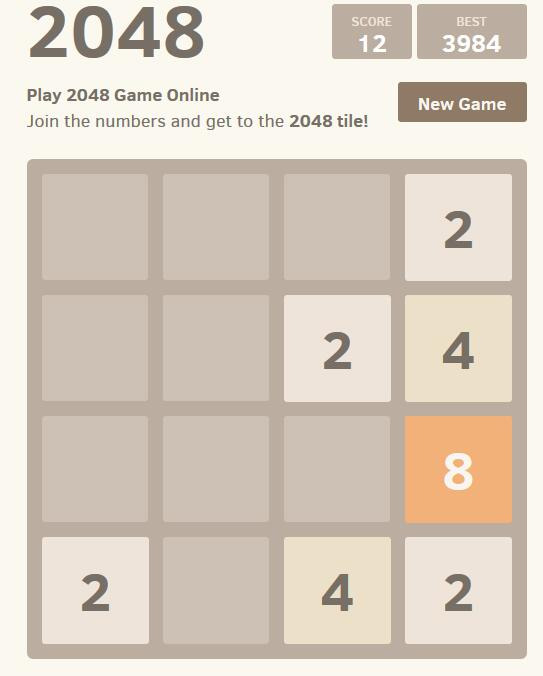
\includegraphics[scale=0.25]{2048_introduction.jpg}
		\caption{"2048"原版游戏界面}
		\label{2048_introduction}
	\end{figure}
	游戏过程中,对所有小块镜像上下左右四个方向的平移。如果平移后有可以合并的小块(即数值相同),则合并为更大数字的小块。以此进行下去。\par
	最后如果有小块达到了2048,则游戏成功;如果已经不能再平移小块了,却还没达到2048,则游戏失败。\par
	\subsection{FPGA版本"2048"游戏界面简介}
	以下是我实现的FPGA版本的游戏界面。有以下几点值得说明:\par
	\keypoint{显示屏上显示的是整个界面,其中原来的数字方块用了一些与中国科学技术大学有关的词汇替代,增加趣味性。}
	\keypoint{充分利用FPGA上的数码管,来显示当前得分。}
	\keypoint{既可以使用NEXYS4开发板上的按键来进行平移和重置游戏,也可以使用键盘上的方向键和回车键实现。}
	\keypoint{游戏进行中的时候,右侧屏幕显示cwk头像;游戏失败时,显示游戏失败的图片;游戏成功时,显示游戏成功的图片。}
	\begin{figure}[H]
		\centering
		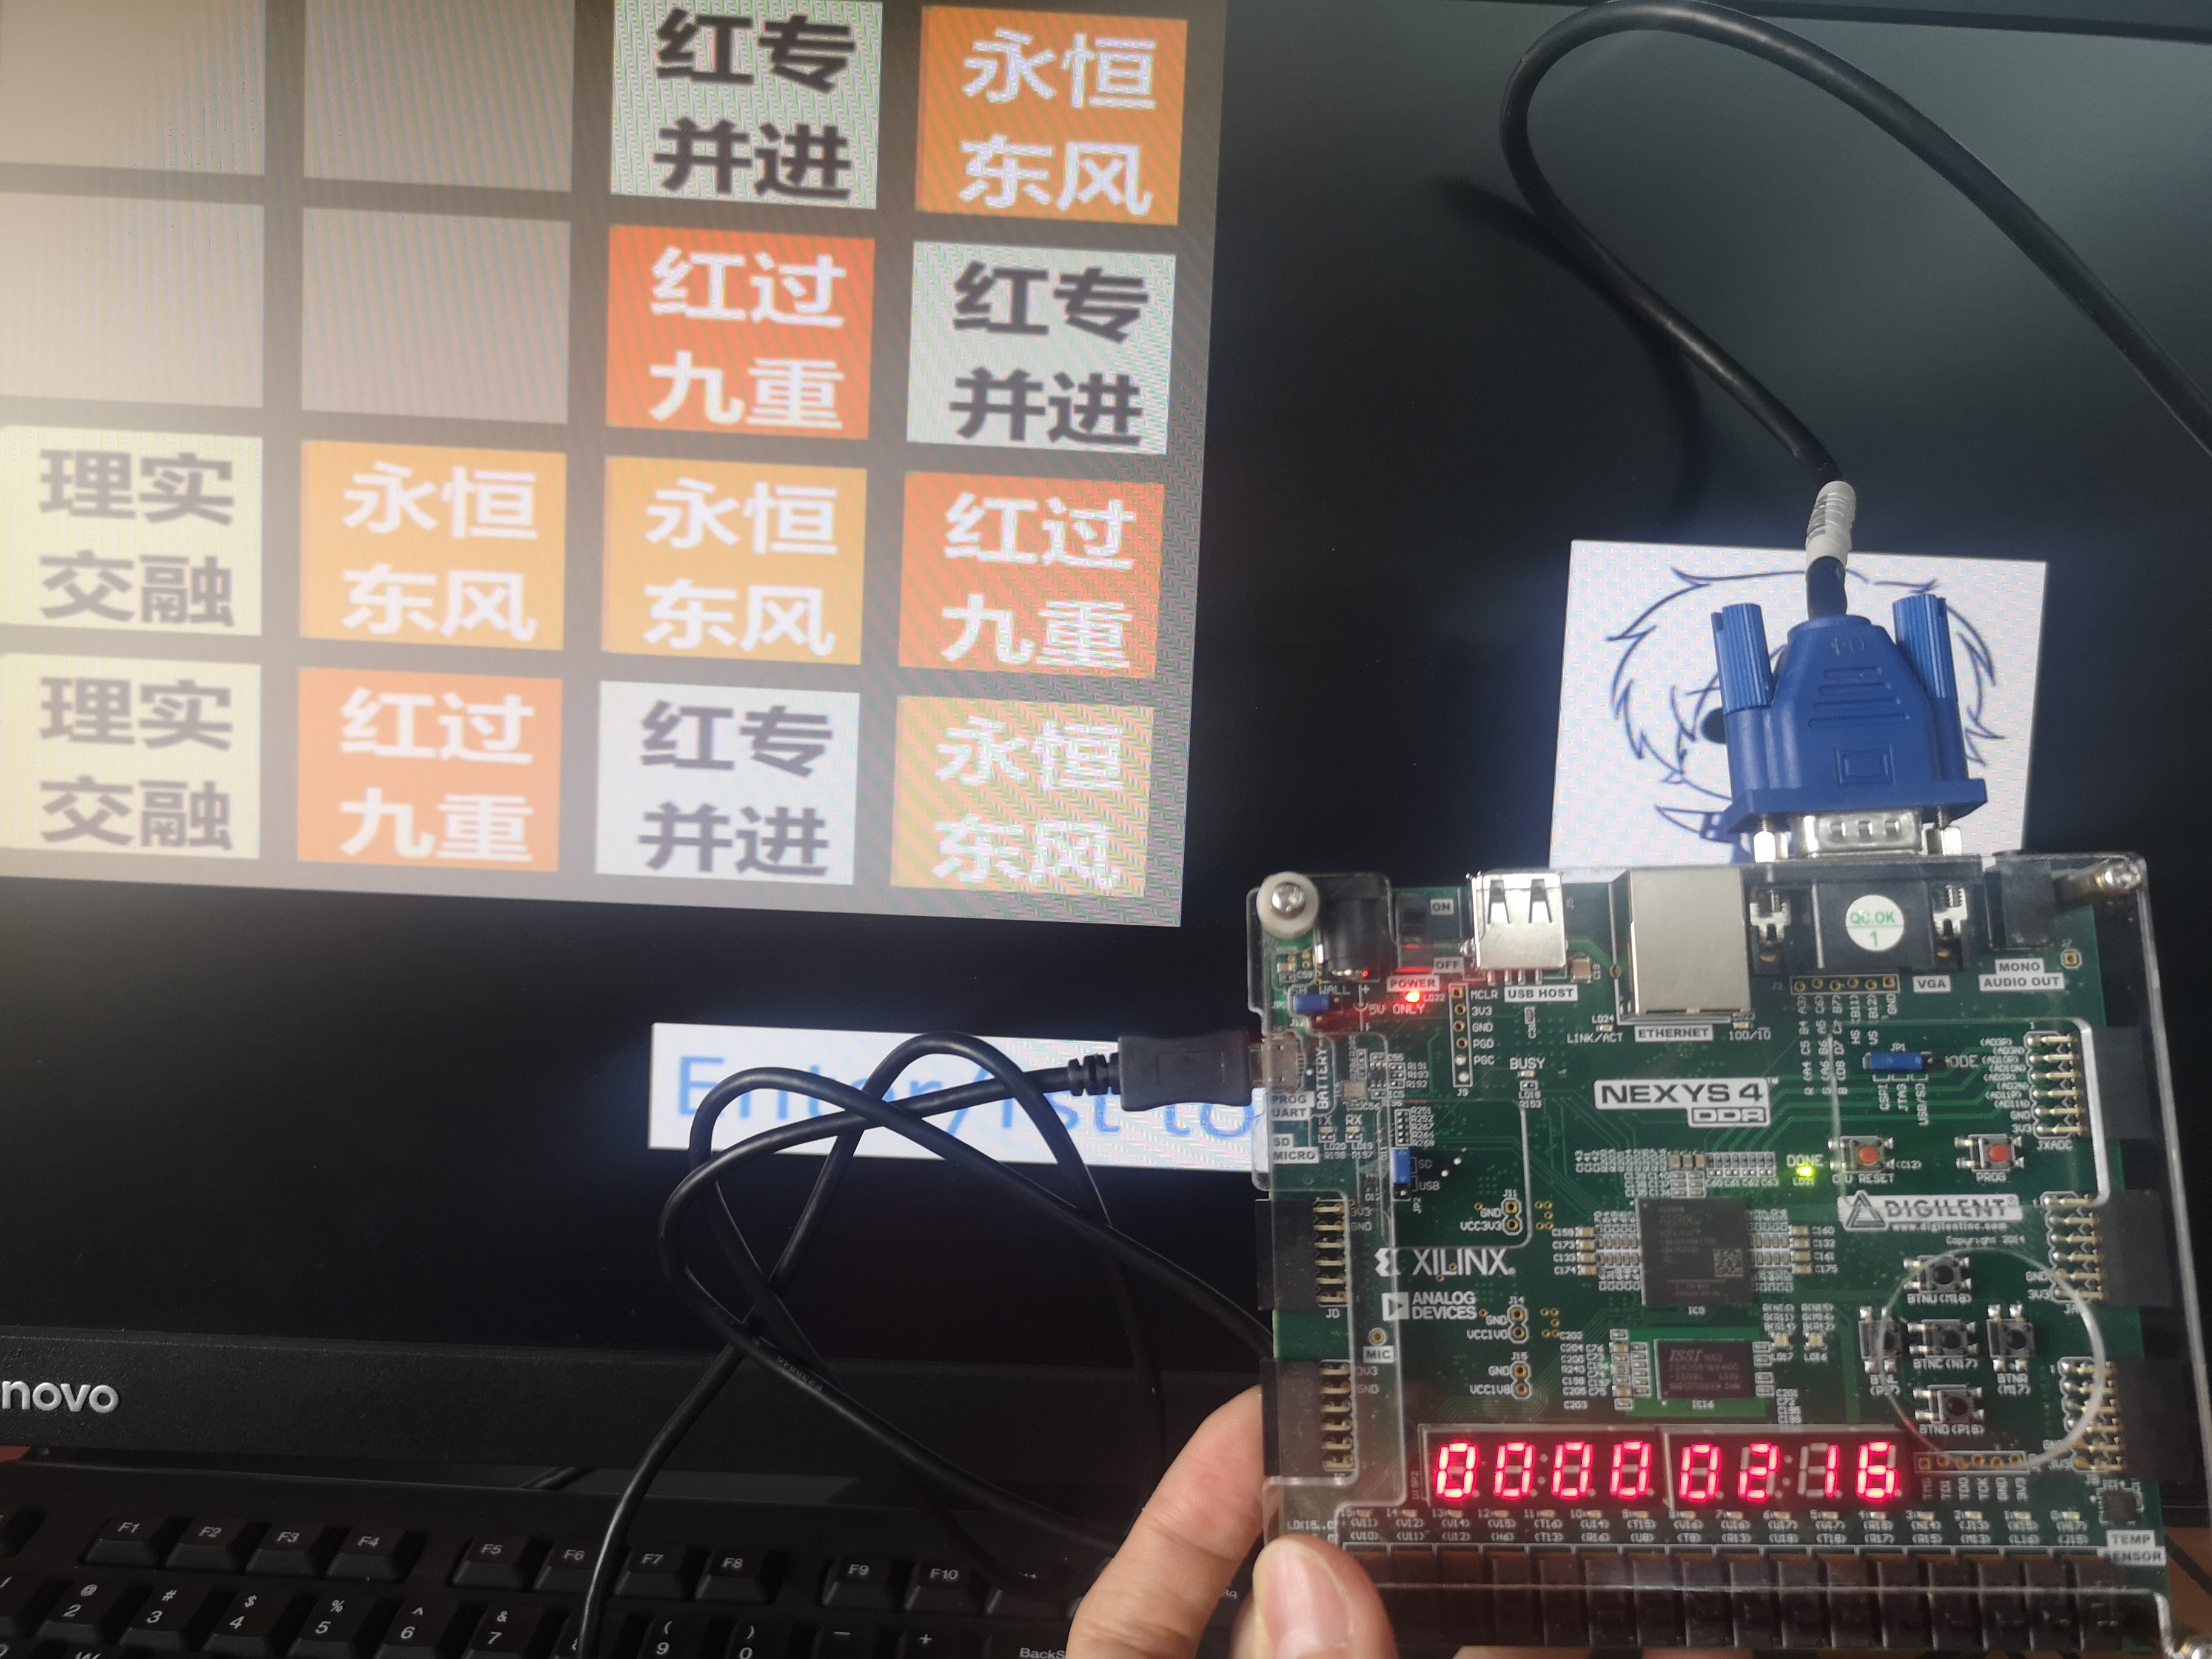
\includegraphics[scale=0.07]{gaming.jpg}
		\caption{FPGA版本"2048"游戏界面}
		\label{gaming}
	\end{figure}\par

	\section{实验项目的具体实现过程}
	本项目具体实现过程主要分为五大块:\par
	\keypoint{第一,VGA显示屏相关模块;}
	\keypoint{第二,上下左右移动模块;}
	\keypoint{第三,PS2键盘输入模块;}
	\keypoint{第四,数码管得分显示模块;}
	\keypoint{第五,游戏状态判定。}
	下面分模块进行介绍。
	\subsection{VGA显示屏模块}
	\subsubsection{VGA显示基本原理}
	首先对VGA显示的基本原理作一个简要介绍。\par
	\begin{figure}[H]
		\begin{minipage}[H]{0.48\linewidth}
			\centering
			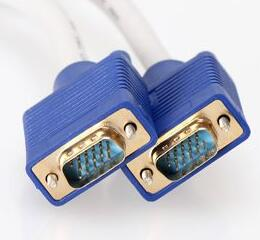
\includegraphics[scale=0.45]{VGA_real_product.jpg}
			\caption{VGA实物图}
			\label{VGA_real_product}
		\end{minipage}
		\quad
		\begin{minipage}[H]{0.48\linewidth}
			\centering
			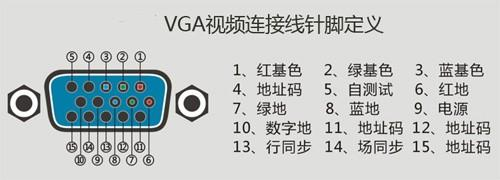
\includegraphics[scale=0.45]{VGA_interface.jpg}
			\caption{VGA接口引脚定义}
			\label{VGA_interface}
		\end{minipage}
	\end{figure}\par
	作为一种视频传输标准的接口,最主要的部分就是它的\textbf{红绿蓝基色引脚}和\textbf{行同步场同步引脚}。\par
	其中颜色的引脚,很显然就是传输了当前扫描的的点应该具有的颜色。那么,行同步和场同步引脚是做什么用的呢?\par
	VGA显示屏的显示方式是按照下面这张图的顺序进行扫描,然后逐点显示不同颜色,最终显示出完整图像的。\par
	\begin{figure}[H]
		\centering
		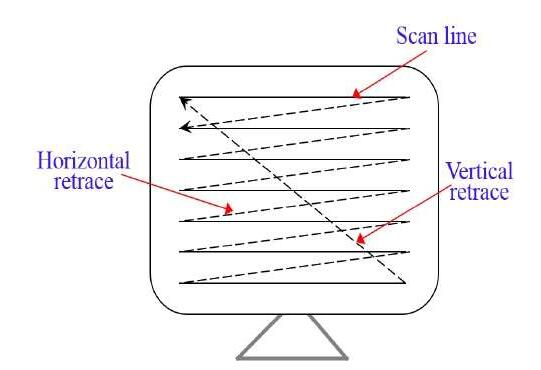
\includegraphics[scale=0.5]{VGA_scan.jpg}
		\caption{VGA扫描过程}
		\label{VGA_scan}
	\end{figure}\par
	那么,在这么复杂的时序下,为了保持同步,就必须引入行同步和场同步信号。其中,每行扫描结束时,用\textbf{行同步信号}进行同步;扫描完所有行后,形成一帧,用\textbf{场同步信号}进行同步。\par
	更为具体的VGA时序图如下:\par
	\begin{figure}[H]
		\centering
		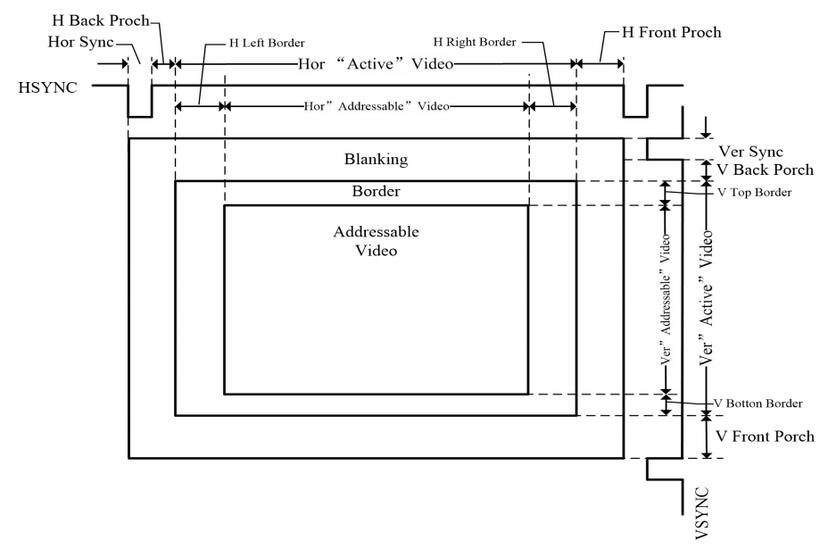
\includegraphics[scale=0.4]{VGA_sequence_chart.jpg}
		\caption{VGA时序图}
		\label{VGA_sequence_chart}
	\end{figure}\par
	总体而言,VGA的时序主要包括行时序和场时序两个部分。二者均主要包含有:行(场)同步、行(场)消隐 、行(场)视频有效和行(场)前肩这四个参数。而不同分辨率的VGA时序中的各个参数,在网上都能轻易地查询得到。\par
	这样,VGA的大致工作原理就介绍完了。下面介绍其代码的实现。\par
	\subsubsection{VGA显示代码实现}
	以下是该模块的输入输出定义。\par
	\begin{lstlisting}[language=Verilog]
	module VGA( 
		input clk,                // 输入时钟信号
		input rst,                // 输入复位信号
		input [1:0] status,       // 游戏状态
		input [63:0] Display_Num,	//游戏小块布局状态
		output reg [3:0] red,    // 输出红色
		output reg [3:0] green,  // 输出绿色
		output reg [3:0] blue,   // 输出蓝色
		output hs,               // 行同步信号
		output vs                // 场同步信号
		);
	\end{lstlisting}\par
	接下来描述其中的代码:\par
	首先,为了使VGA能按特定的参数进行扫描,需要生成对应的行、场时序。下面简单对行时序的产生进行解析。\par
	为了生成行时序,应该有一个计数器h\_cnt,当它计数到行末尾的时候,便重新返回0,否则不断自加。此外,还应该在对应时候产生行同步信号hs,其中hs作为output连接到VGA接口上。\par
	\begin{lstlisting}[language=Verilog]
	// 生成行时序
	always @(posedge clk_65M)
	begin
		if(h_cnt == H_LINE_PERIOD - 1'b1) //计数到行末,返0
			h_cnt <= 12'd0;
		else //正常计数,自加
			h_cnt <= h_cnt + 1;
	end
	assign hs = (h_cnt < H_SYNC_PULSE) ? 1'b0 : 1'b1;  //行同步信号产生
	\end{lstlisting}\par
	至于场同步时序部分代码可参见附录。\par
	\jumpline
	
	其次,要想在屏幕上显示图像,只有行、场同步时序是不够的。我们还需要对颜色进行输出。\par
	思路也很简单,就是对h\_cnt和v\_cnt的扫描到的位置进行一个判断,如果在要显示图片的范围内,就显示图片的对应像素点。而为了能显示图片,我使用了IP核\textbf{"Block Memory Generator"}来保存对应图片。而这里用到的COE文件转换,我借助了Python对图像的处理工具来完成。(代码附于附录中)下面取显示某一张图片的部分代码介绍。具体代码及注释如下:\par
	\begin{lstlisting}[language=Verilog, name=一些变量的声明]
	//显示图片的位置和大小信息
	parameter IMAGE_START_H = 668;
	parameter IMAGE_START_V = 284;
	parameter IMAGE_WIDTH = 200;
	parameter IMAGE_HEIGHT = 200;
	parameter IMAGE_PIX_NUM = 40000;
	
	reg [15:0] rom_addr; //图片中的地址
	wire [11:0] rom_data; //图片中的地址对应的颜色信息
	// 图片IP核的例化
	img_cwk img_cwk(.addra(rom_addr),.clka(clk_65M),.douta(rom_data),.ena(1'b1)); 
	\end{lstlisting}\par
	\jumpline
	\begin{lstlisting}[language=Verilog, name=图片显示的部分]
	// 判断当前h_cnt和v_cnt是否已经计数到图片显示的范围
	if(h_cnt >= (H_SYNC_PULSE + H_BACK_PORCH + IMAGE_START_H)  &&
		h_cnt <= (H_SYNC_PULSE + H_BACK_PORCH + IMAGE_WIDTH-1'b1 + IMAGE_START_H)  && 
		v_cnt >= (V_SYNC_PULSE + V_BACK_PORCH + IMAGE_START_V)  &&
		v_cnt <= (V_SYNC_PULSE + V_BACK_PORCH + IMAGE_HEIGHT-1'b1 + IMAGE_START_V))
	begin
		// 如果是,判断游戏状态,
		if(status == gaming) //若是游戏进行中,则显示rom_addr和rom_data对应的图片
		begin
			rom_addr_fail <=  15'd0 ; //其他图片显示的addr寄存器置0
			rom_addr_success <=  15'd0 ; //其他图片显示的addr寄存器置0
			red <= rom_data[11:8]; // 红色分量
			green <= rom_data[7:4]; // 绿色分量
			blue <= rom_data[3:0]; // 蓝色分量
			if(rom_addr == IMAGE_PIX_NUM - 1'b1) //将本图片的addr寄存器自加,直到最后一个像素点
				rom_addr  <=  15'd0 ; //到了最后一个像素点,则置0
			else
				rom_addr  <=  rom_addr  +  1'b1;  //否则addr自加
		end
		//以下略去
		//...
	end
	\end{lstlisting}\par
	\jumpline
	最后,对我认为VGA模块部分最困难的显示,即游戏中16个小块的显示,作一个简要介绍。\par
	其中,用\textbf{input [63:0] Display\_Num}作为该模块的一个输入,它是对16个方块显示的图片的编码。例如,第0行第0列的方块,则是用Display\_Num[3:0]表示,如果这个值是$n$,则显示$2^{n}$对应的小块图片。\par
	下面以(0,0)块的显示为例作说明:\par
	\begin{lstlisting}[language=Verilog, name=各个小块的显示]
	//以(0,0)块为例
	//判断h_cnt和v_cnt是否在(0,0)块范围内
	if(
		h_cnt >= (H_SYNC_PULSE + H_BACK_PORCH - BLOCK_WIDTH + FRAME_START_H_1) &&
		h_cnt <= (H_SYNC_PULSE + H_BACK_PORCH - 1'b1 + FRAME_START_H_1) && 
		v_cnt >= (V_SYNC_PULSE + V_BACK_PORCH - BLOCK_WIDTH + FRAME_START_V_1) &&
		v_cnt <= (V_SYNC_PULSE + V_BACK_PORCH - 1'b1 + FRAME_START_V_1))
	begin
		//如果是,则做对应显示
		rom_addr_num_input <= rom_addr_num[0];
		{red, green, blue} <= rom_data_num[Display_Num[3:0]];
		if(rom_addr_num[0] == BLOCK_PIX_NUM - 1'b1) 
			rom_addr_num[0] <=  12'd0;
		else 
			rom_addr_num[0] <=  rom_addr_num[0] + 1'b1;
	end
	\end{lstlisting}\par
	\jumpline
	此外,其实还有一些边框,背景等的显示,都大同小异,故不再赘述,详见附录代码。\par
	
	\subsection{平移模块}
	游戏过程中,需要有平移的操作。为了完成平移,我构建了4个方向的module。下面以Up\_Move上移模块为例进行介绍。\par
	\subsubsection{模块的输入输出定义}
	其输入输出定义如下:\par
	\begin{lstlisting}[language=Verilog, name=平移模块输入输出定义]
	module Up_Move(
		input rst,	//复位
		input clk,	//时钟信号
		input Signal,	//按键触发信号
		input key,		//键盘触发信号
		input [63:0] input_state,	//当前游戏小块状态
		output reg [63:0] Display_Num,	//经过移动后,小块状态信号
		output ok	//平移处理完成信号
		);
	\end{lstlisting}\par
	\subsubsection{对输入预处理——去抖动和边沿}
	下面,首先应该对输入进行一些预处理。
	其中,既然有输入,则不可避免地会有抖动,因此有如下相应去抖动代码:\par
	\begin{lstlisting}[language=Verilog, name=输入去抖动]
	//去抖动
	always @(posedge clk)
	begin
		if(Signal)
		begin
			if(Signal_counter >= 100000) //计数到这个值才认为是输入有效
			begin
				Signal_counter <= 100000;        
				Signal_0 <= 1;
			end
			else //否则继续计数
				Signal_counter <= Signal_counter + 1;
		end
		else //其他情况则初始化
		begin
			Signal_counter <= 0;
			Signal_0 <= 0;
		end
	end
	\end{lstlisting}\par
	此外,根据游戏的特性,应该对输入取边缘信号:\par
	\begin{lstlisting}[language=Verilog, name=输入取边缘]
	//取边缘
	reg Signal_0, Signal_1, Signal_2;
	wire Signal_Redge;
	always @(posedge clk) Signal_1 <= Signal_0;
	always @(posedge clk) Signal_2 <= Signal_1;
	assign Signal_Redge = Signal_1 & ~Signal_2;
	\end{lstlisting}\par
	\jumpline
	\subsubsection{正式平移}
	完成了对输入的预处理,则可以根据输入进行平移。平移过程分为三个部分:第一,沿着对应方向把小块平移,先不进行合并;第二,针对几种不同情况,对小块的合并分类处理;第三,随机生成新的小块。\par
	\textbf{第一部分:初步平移}\par
	\begin{lstlisting}[language=Verilog, name=初步平移]
	//先把方块平移到补齐最下面一格
	if(last_state[3:0] == 4'h0) 
	begin 
		last_state[3:0] = last_state[19:16]; last_state[19:16] = last_state[35:32]; 
		last_state[35:32] = last_state[51:48]; last_state[51:48] = 0; 
	end
	if(last_state[3:0] == 4'h0) 
	begin 
		last_state[3:0] = last_state[19:16]; last_state[19:16] = last_state[35:32]; 
		last_state[35:32] = last_state[51:48]; last_state[51:48] = 0; 
	end
	if(last_state[3:0] == 4'h0) 
	begin 
		last_state[3:0] = last_state[19:16]; last_state[19:16] = last_state[35:32]; 
		last_state[35:32] = last_state[51:48]; last_state[51:48] = 0; 
	end
	if(last_state[3:0] == 4'h0) 
	begin 
		last_state[3:0] = last_state[19:16]; last_state[19:16] = last_state[35:32]; 
		last_state[35:32] = last_state[51:48]; last_state[51:48] = 0; 
	end
	//再补齐倒数第二格
	if(last_state[19:16] == 4'h0) 
	begin 
		last_state[19:16] = last_state[35:32]; last_state[35:32] = last_state[51:48]; last_state[51:48] = 0; 
	end
	begin 
		last_state[19:16] = last_state[35:32]; last_state[35:32] = last_state[51:48]; last_state[51:48] = 0; 
	end
	begin 
		last_state[19:16] = last_state[35:32]; last_state[35:32] = last_state[51:48]; last_state[51:48] = 0; 
	end
	//最后补齐倒数第三格
	if(last_state[35:32] == 4'h0) 
	begin 
		last_state[35:32] = last_state[51:48]; last_state[51:48] = 0; 
	end
	if(last_state[35:32] == 4'h0) 
	begin 
		last_state[35:32] = last_state[51:48]; last_state[51:48] = 0; 
	end
	\end{lstlisting}\par
	\jumpline
	\textbf{第二部分:合并}\par
	合并的时候,只有下面四种情况需要考虑。\par
	\keypoint{第一行和第二行的相同,第三行和第四行的相同,且不为0}
	\keypoint{第一行和第二行的相同,且不为0}
	\keypoint{第三行和第四行的相同,且不为0}
	\keypoint{第二行和第三行的相同,且不为0}
	\begin{figure}[H]
		\begin{minipage}[H]{0.36\linewidth}
			\centering
			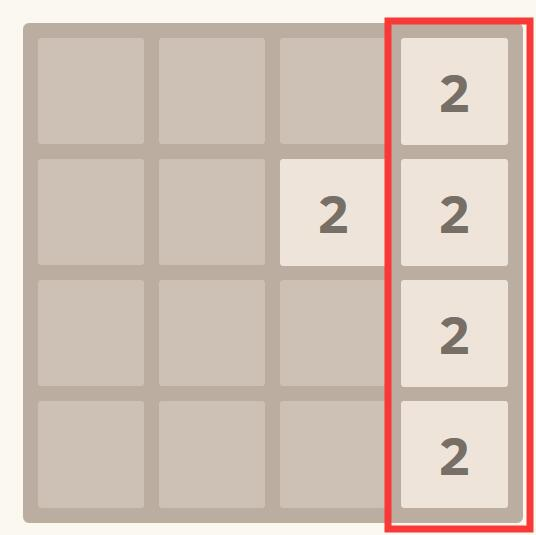
\includegraphics[scale=0.30]{12_34.jpg}
			\caption{第一行和第二行的相同,第三行和第四行的相同,且不为0}
			\label{12_34}
		\end{minipage}
		\qquad
		\begin{minipage}[H]{0.36\linewidth}
			\centering
			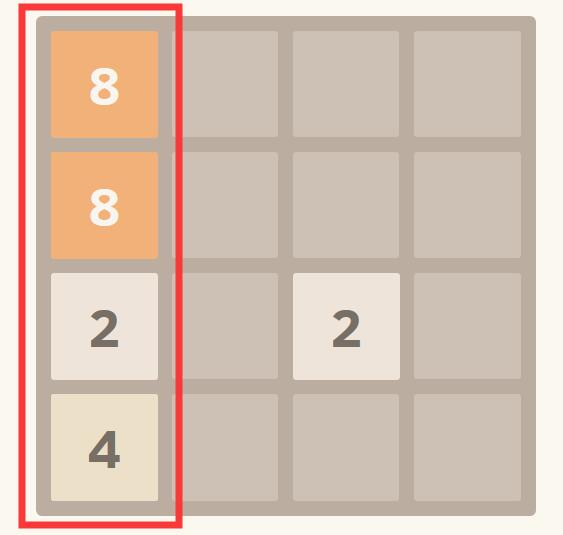
\includegraphics[scale=0.30]{12.jpg}
			\caption{第一行和第二行的相同,且不为0}
			\label{12}
		\end{minipage}
	\end{figure}
	\begin{figure}[H]
		\begin{minipage}[H]{0.36\linewidth}
			\centering
			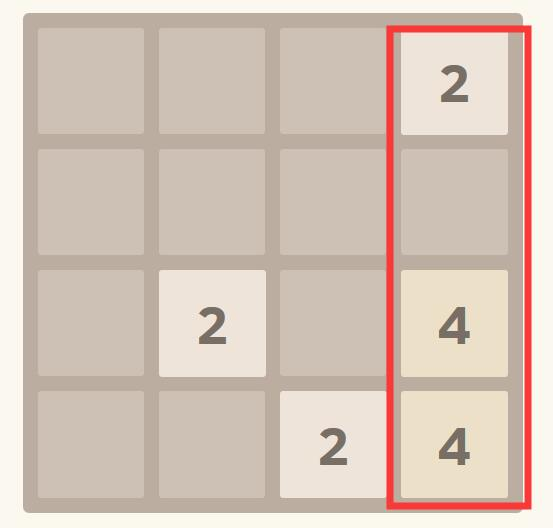
\includegraphics[scale=0.30]{34.jpg}
			\caption{第三行和第四行的相同,第三行和第四行的相同,且不为0}
			\label{34}
		\end{minipage}
		\qquad
		\begin{minipage}[H]{0.36\linewidth}
			\centering
			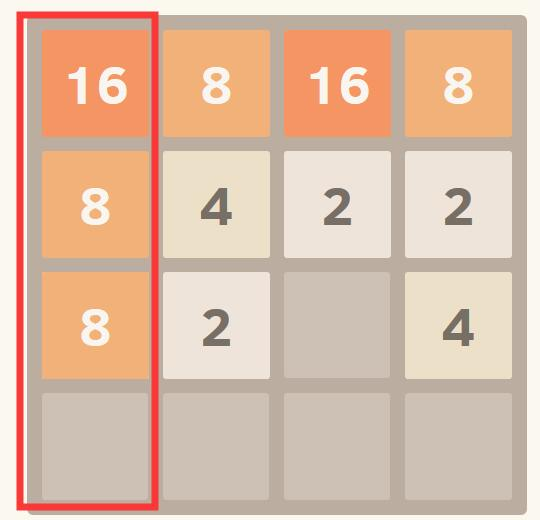
\includegraphics[scale=0.30]{23.jpg}
			\caption{第二行和第三行的相同,且不为0}
			\label{23}
		\end{minipage}
	\end{figure}
	按照上述分类,对合并后的状态赋值即可。代码及注释如下:\par
	\begin{lstlisting}[language=Verilog, name=方块合并]
	//然后对方块的合并做处理
	//第一行和第二行的相同,第三行和第四行的相同,且不为0
	if(last_state[3:0] == last_state[19:16] && last_state[35:32] == last_state[51:48]
	&& last_state[51:48] != 0 && last_state[19:16] != 0)
	begin
		last_state[3:0] = last_state[3:0] + 4'h1;
		last_state[19:16] = last_state[19:16] + 4'h1;
		last_state[35:32] = 4'h0; last_state[51:48] = 4'h0;
	end
	//第一行和第二行的相同,且不为0
	else if(last_state[3:0] == last_state[19:16] && last_state[19:16] != 0)
	begin
		last_state[3:0] = last_state[3:0] + 4'h1;
		last_state[19:16] = last_state[35:32];
		last_state[35:32] = last_state[51:48]; 
		last_state[51:48] = 4'h0;
	end
	//第三行和第四行的相同,且不为0
	else if(last_state[19:16] == last_state[35:32] && last_state[19:16] != 0)
	begin
		last_state[19:16] = last_state[19:16] + 4'h1;
		last_state[35:32] = last_state[51:48];
		last_state[51:48] = 4'h0;
	end
	//第二行和第三行的相同,且不为0
	else if(last_state[35:32] == last_state[51:48] && last_state[51:48] != 0)
	begin
		last_state[35:32] = last_state[35:32] + 4'h1; 
		last_state[51:48] = 4'h0;
	end
	//对第一列的处理结束
	\end{lstlisting}\par
	\jumpline
	\textbf{第三部分:随机生成新小块}\par
	这里随机生成的方式是采用一个计数器,每次时钟边缘都让计数器自加,当按下操作的时候,则在计数器对应的位置生成新的小块。若对应位置已经有小块,则在其顺序数下去的第一个空位置生成小块。\par
	随机数的计数器及计数代码如下:\par
	\begin{lstlisting}[language=Verilog, name=随机数的计数器]
	reg [1:0] random_counter = 0;
	//每次时钟边缘则自加
	always @(posedge clk)
	begin
		random_counter <= random_counter + 2'h1;
	end
	\end{lstlisting}\par
	而随机小块生成的代码如下:\par
	\begin{lstlisting}[language=Verilog]
	//根据随机计数器random_counter新生成一个方块2,开始
	//只有当移动有效(即移动前后状态不同),才会生成新的小块
	if(last_state != input_state)
	begin
		//进一步判断可否在该位置生成,否则顺延
		if(random_counter == 2'h0) 
		begin
			if(last_state[51:48] == 4'h0) last_state[51:48] = 4'h1;
			else if(last_state[55:52] == 4'h0) last_state[55:52] = 4'h1;
			else if(last_state[59:56] == 4'h0) last_state[59:56] = 4'h1;
			else if(last_state[63:60] == 4'h0) last_state[63:60] = 4'h1;
			else last_state = last_state;
		end
		//进一步判断可否在该位置生成,否则顺延
		else if(random_counter == 2'h1) 
		begin
			if(last_state[55:52] == 4'h0) last_state[55:52] = 4'h1;
			else if(last_state[59:56] == 4'h0) last_state[59:56] = 4'h1;
			else if(last_state[63:60] == 4'h0) last_state[63:60] = 4'h1;
			else if(last_state[51:48] == 4'h0) last_state[51:48] = 4'h1;
			else last_state = last_state;
		end
		//进一步判断可否在该位置生成,否则顺延
		else if(random_counter == 2'h2) 
		begin
			if(last_state[59:56] == 4'h0) last_state[59:56] = 4'h1;
			else if(last_state[63:60] == 4'h0) last_state[63:60] = 4'h1;
			else if(last_state[51:48] == 4'h0) last_state[51:48] = 4'h1;
			else if(last_state[55:52] == 4'h0) last_state[55:52] = 4'h1;
			else last_state = last_state;
		end
		//进一步判断可否在该位置生成,否则顺延
		else if(random_counter == 2'h3) 
		begin
			if(last_state[63:60] == 4'h0) last_state[63:60] = 4'h1;
			else if(last_state[51:48] == 4'h0) last_state[51:48] = 4'h1;
			else if(last_state[55:52] == 4'h0) last_state[55:52] = 4'h1;
			else if(last_state[59:56] == 4'h0) last_state[59:56] = 4'h1;
			else last_state = last_state;
		end
		else last_state = last_state;
	end
	else last_state = last_state;
	//根据随机计数器random_counter新生成一个方块2,结束
	\end{lstlisting}\par
	\jumpline
	其余部分则是对一些诸如复位等的特别情况的处理,在此不再赘述,详见附录代码。\par

	\subsection{PS2键盘输入模块}
	\subsubsection{PS2键盘输入原理和时序介绍}
	在Nexys4开发板上,键盘的使用是按照PS2接口时序完成的。它的接口引脚定义如下:\par
	\begin{figure}[H]
		\centering
		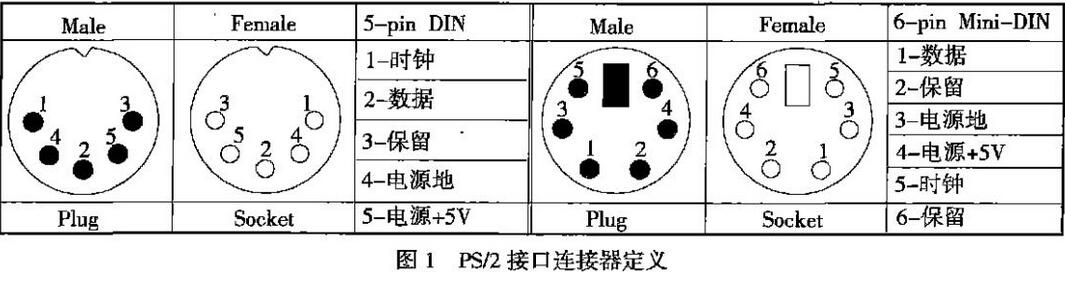
\includegraphics[scale=0.5]{PS2_interface.jpg}
		\caption{PS2接口引脚定义}
		\label{PS2_interface}
	\end{figure}\par
	它可以实现双向传输。这里用键盘,主要使用的是键盘向开发板的数据传输。PS2 设备向主机发送数据时, 会首先检测时钟信号是否为高电平,然后连续发送 11 个时钟负脉冲,并在数据线上发送 11bit 的数据,包括起始位(1bit)、数据位(8bit)、校验位(1bit)和停止位(1bit),主机可在 PS2\_CLK 信号的下降沿对数据信号进行采样,其时序图如下所示:
	\begin{figure}[H]
		\centering
		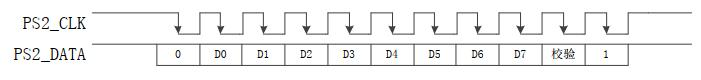
\includegraphics[scale=0.5]{PS2_sequence_chart.jpg}
		\caption{PS2时序图}
		\label{PS2_sequence_chart}
	\end{figure}\par
	对于这种工作模式,键盘上按键被按下和松开时都会有数据传输。例如当’a’被按下时,发送一个字节“1C”(称为通码),该按键松开时,发送两个字节“F0 1C”(称为断码)。\par
	而真正我们使用它的时候,只需要取11 bits中的8个有效bit。\par
	但不幸的是,由于现在市面上的键盘大多已经不再是PS2的接口,而是USB型的。虽然Nexys4开发板对这种键盘也有一定兼容,但我尝试了包括自己的,实验室里的等键盘,都无法正常在PS2的模式下工作。所幸后来借到了一位同学的一个比较旧的键盘,恰好是可以正常工作的。\par
	\subsubsection{PS2键盘输入代码}
	该模块的输入输出定义如下:\par
	\begin{lstlisting}[language=Verilog, name=PS2输入输出定义]
	module Keyboard(
		input clk,  //时钟信号
		input rst,  //复位信号
		input ps2_clk,  //PS2时钟信号
		input ps2_data, //PS2数据信号
		output reg	[3:0] LED,   //方向键按下信号
		output reg enter    //回车键按下信号
		);
	\end{lstlisting}
	以下是PS2键盘输入的关键部分:\par
	\begin{lstlisting}[language=Verilog, name=PS2输入数据关键代码]
	always@(posedge clk or posedge rst) 
	begin
		if(rst)
			key <= 16'hFFFF;
		else if(ps2_clk_neg) //由PS2时钟信号确认工作状态
		begin
			//如果输入对应的8个数据位,则存入寄存器key中
			if((ps2_clk_cnt>=1)&&(ps2_clk_cnt<=8)) 
				key <= {ps2_data,key[15:1]};   
			else //否则key保持不变
				key <= key;
		end
	end
	\end{lstlisting}
	其他还有一些时序状态计数等的内容,相对简单,囿于篇幅,就不再展示了。可参见附录。
	
	\subsection{数码管模块}
	\subsubsection{数码管模块}
	数码管是通过对不同位置的灯赋予高低电平以点亮,并通过时分复用的方式来完成多位同时显示的效果的。\par
	它的原理相对简单,故直接对代码稍作解释。如下:\par
	首先是模块的输入输出定义:\par
	\begin{lstlisting}[language=Verilog]
	module Nixietube(
		input clk, rst, //时钟信号,复位信号
		input [26:0] x, //输入二进制数
		output reg [7:0] seg,   //输出数码管的显示
		output reg [7:0] AN     //输出数码管的选择
		);
	\end{lstlisting}
	此外的关键部分:二进制转换为十进制的代码如下:\par
	\begin{lstlisting}[language=Verilog, name=二进制数转换为十进制]
	// 计算dec
	// 采用加3移位法
	always @(posedge clk or posedge rst)
	begin
		if(rst)
			dec = 0;
		else 
		begin
			if(counter == 32'd100000)
			begin
				dec = 0;
				dec[26:0] = x;
				//重复27次加三移位法,27是二进制数的位数
				repeat(27)
				begin
					//
					if(dec[58:55] >= 5 || dec[54:51] >= 5 || dec[50:47] >= 5 || dec[46:43] >= 5 || dec[42:39] >= 5 || dec[38:35] >= 5 || dec[34:31] >= 5 || dec[30:27] >= 5)
					begin
						if(dec[58:55] >= 5) dec[58:55] = dec[58:55] + 3;
						if(dec[54:51] >= 5) dec[54:51] = dec[54:51] + 3;
						if(dec[50:47] >= 5) dec[50:47] = dec[50:47] + 3;
						if(dec[46:43] >= 5) dec[46:43] = dec[46:43] + 3;
						if(dec[42:39] >= 5) dec[42:39] = dec[42:39] + 3;
						if(dec[38:35] >= 5) dec[38:35] = dec[38:35] + 3;
						if(dec[34:31] >= 5) dec[34:31] = dec[34:31] + 3;
						if(dec[30:27] >= 5) dec[30:27] = dec[30:27] + 3;
					end
					dec = dec << 1;
				end
			end
		end
	end
	\end{lstlisting}
	至于时分复用等其他部分的代码都比较简单,请详见附录。\par
	
	\subsection{游戏状态判定部分}
	\subsubsection{得分显示}
	利用上述数码管模块即可显示得分。由数学归纳法可以发现,场上一个$2^{n}$的方块,分值应为$scores(n)=scores(n-1)\times 2+2^{n}$,通过这个递推式可以确定任意一种小块的分值。因此只需要可以统计场上小块,就能给出总分。\par
	\begin{lstlisting}[language=Verilog, name=得分统计]
	reg [26:0] scores;
	wire [26:0] toAdd [15:0]; 
	Nixietube(.clk(clk), .rst(rst), .x(scores), .seg(seg), .AN(AN));
	dist_mem_gen_0 dist_mem_gen_0_0(.a(Display_Num[3:0]), .spo(toAdd[0]));
	dist_mem_gen_0 dist_mem_gen_0_1(.a(Display_Num[7:4]), .spo(toAdd[1]));
	//这里省略了其他的例化
	always @(posedge clk)
	begin
		scores <= toAdd[0] + toAdd[1] + toAdd[2] + toAdd[3] + toAdd[4] + toAdd[5] + toAdd[6] + toAdd[7] + toAdd[8] + toAdd[9] + toAdd[10] + toAdd[11] + toAdd[12] + toAdd[13] + toAdd[14] + toAdd[15];
	end
	\end{lstlisting}
	\subsubsection{游戏状态}
	这个游戏需要判断每次移动后,是否达到游戏成功,游戏失败,或仍然是正在游戏过程中。\par
	观察可知,游戏成功的条件是:存在小块值达到2048;游戏失败的条件是:所有小块都非空,且相邻小块不同;否则,正在游戏过程中\par
	判断语句可以这样写:\par
	\begin{lstlisting}[language=Verilog, name=游戏状态判定部分代码]
	//注:这不是完整代码
	//用这样的语句判断(0,0)小块是否达到目标值
	Display_Num[3:0] == target
	
	//用这样的语句判断(0,0)小块是否达非空
	Display_Num[3:0] != 4'h0
	
	//用这样的语句判断(0,0)小块和(0,1)小块是否相同
	Display_Num[3:0] != Display_Num[7:4]
	\end{lstlisting}
	
	
	\section{实验项目成果展示}
	在游戏过程中,形成了如下的界面:\par
	\begin{figure}[H]
		\centering
		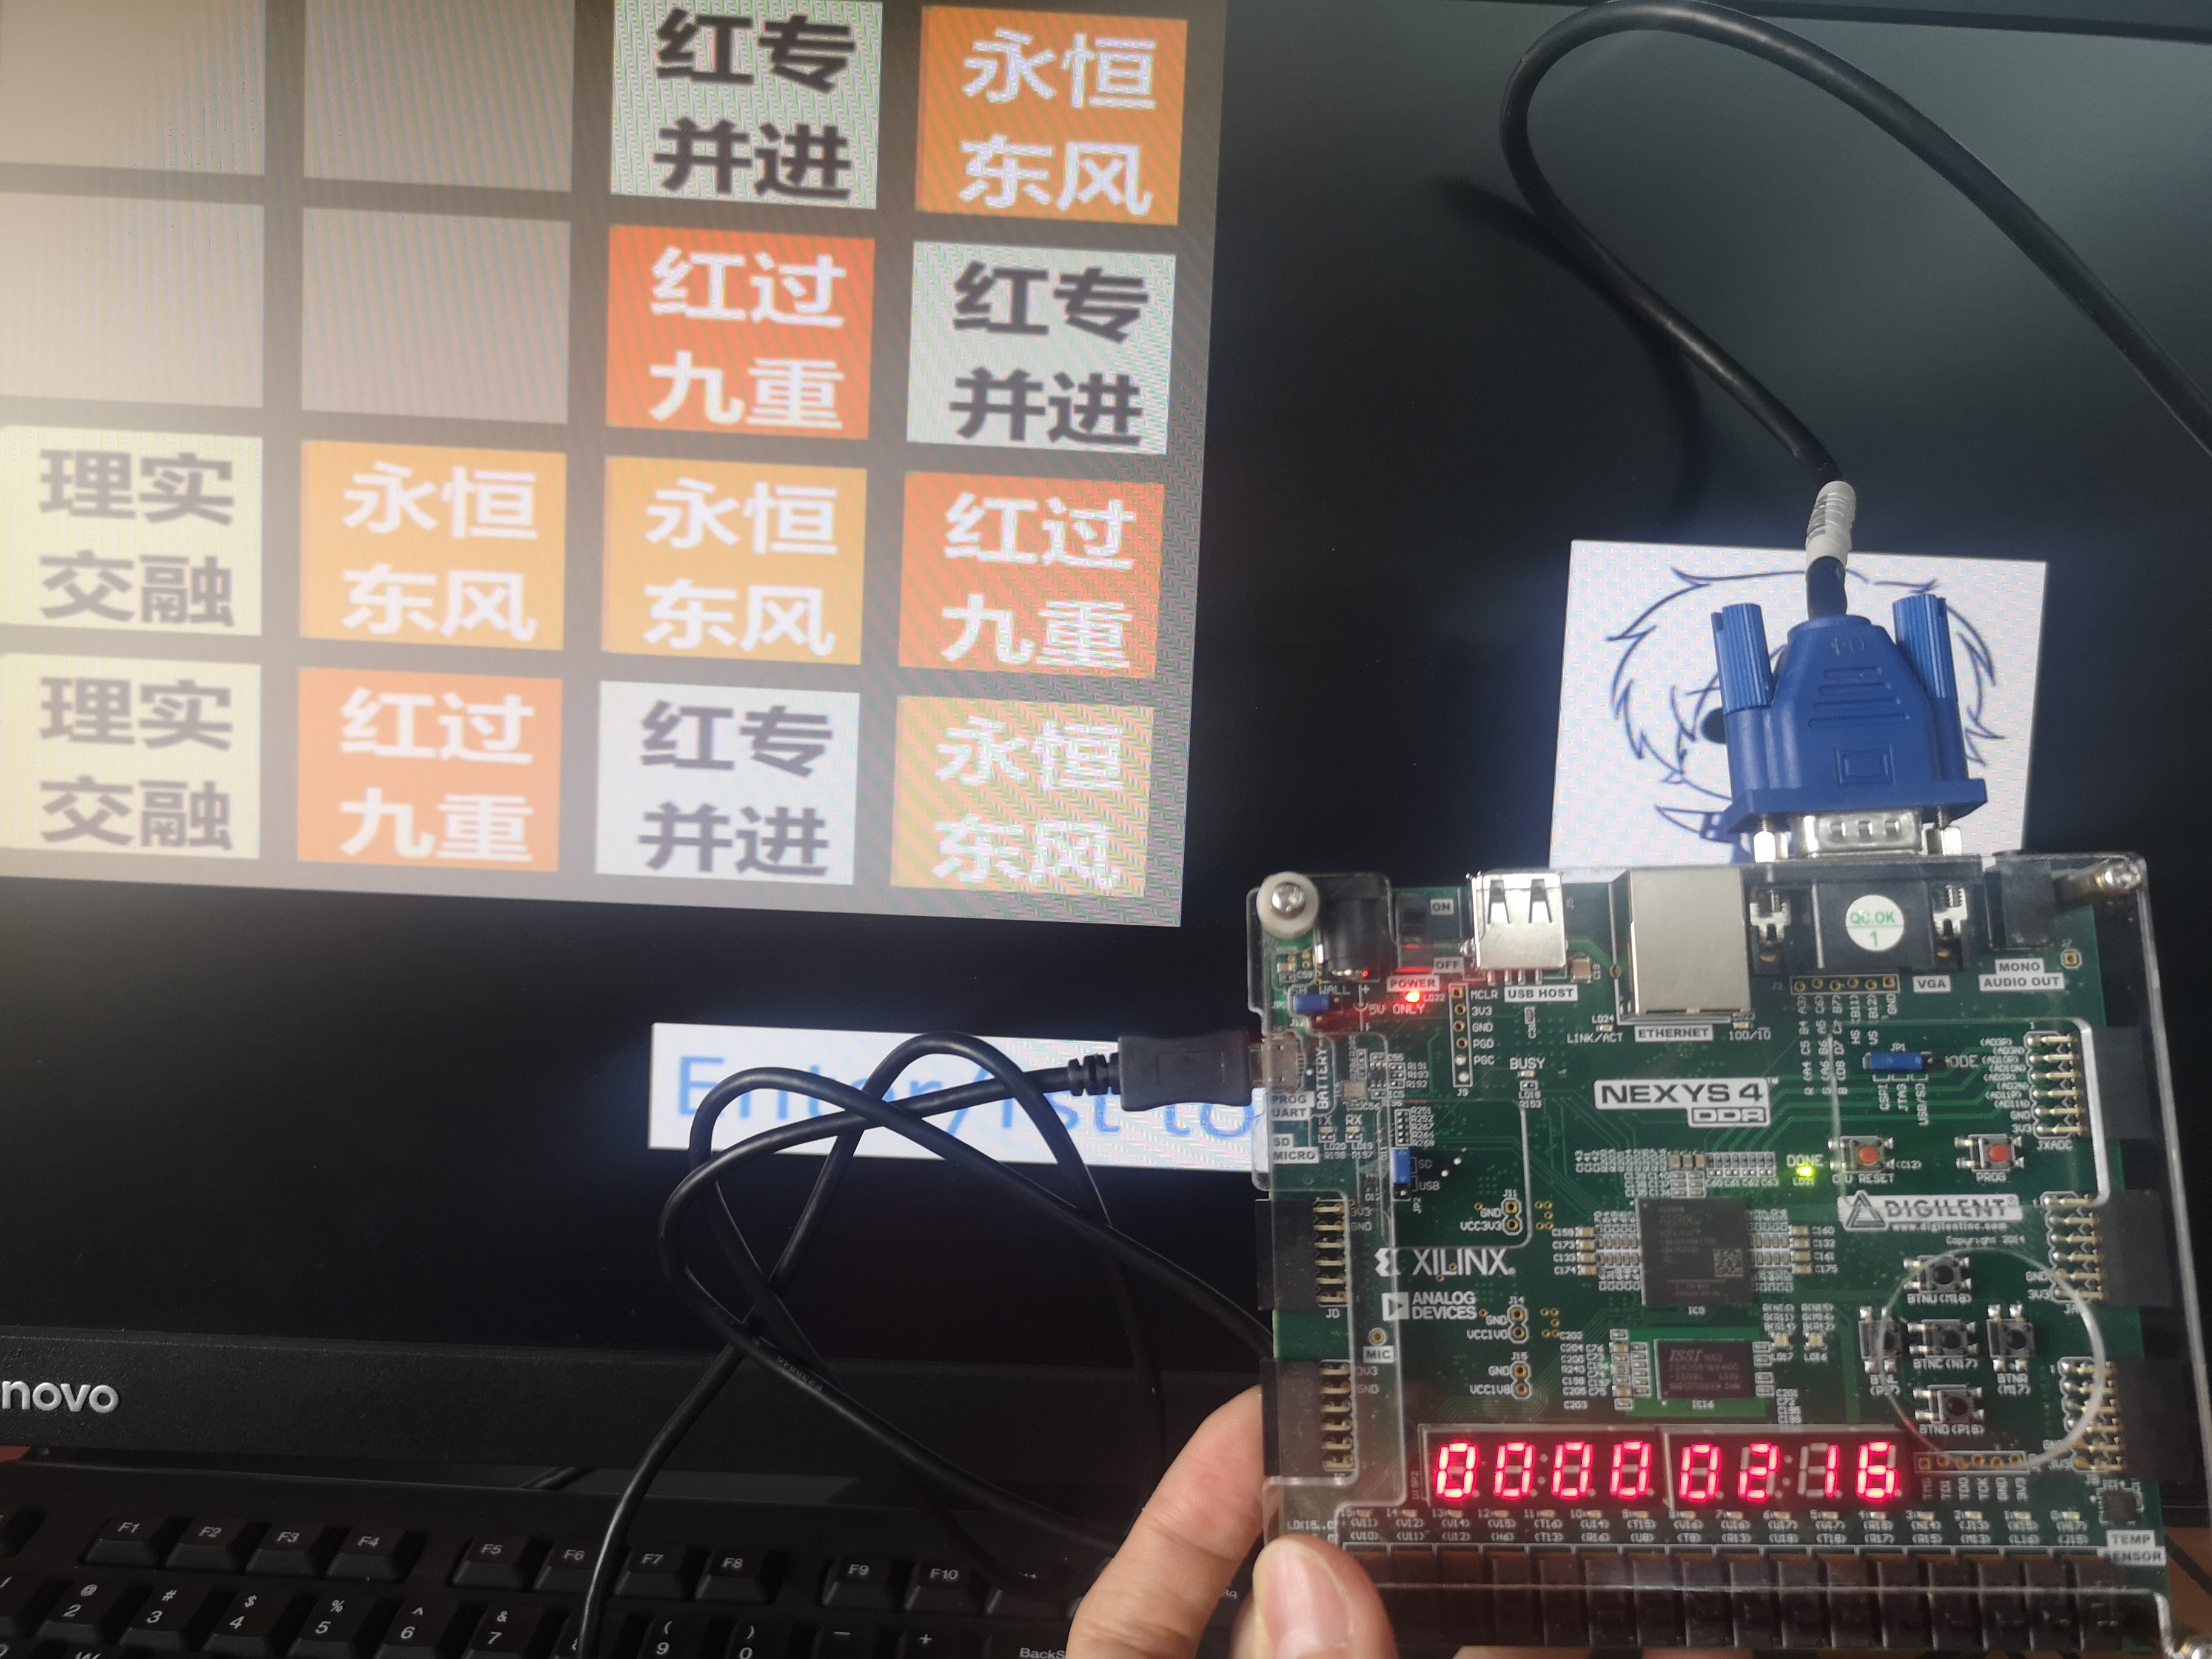
\includegraphics[scale=0.07]{gaming.jpg}
		\caption{FPGA版本"2048"游戏界面}
		\label{gaming}
	\end{figure}\par
	可以看到,显示屏上显示了各个小块,且旁边有小图片来指示游戏的状态(游戏中,游戏成功,游戏失败);在FPGA上也有数码管显示得分情况。
	而当游戏失败的时候,画面如下:\par
	\begin{figure}[H]
		\centering
		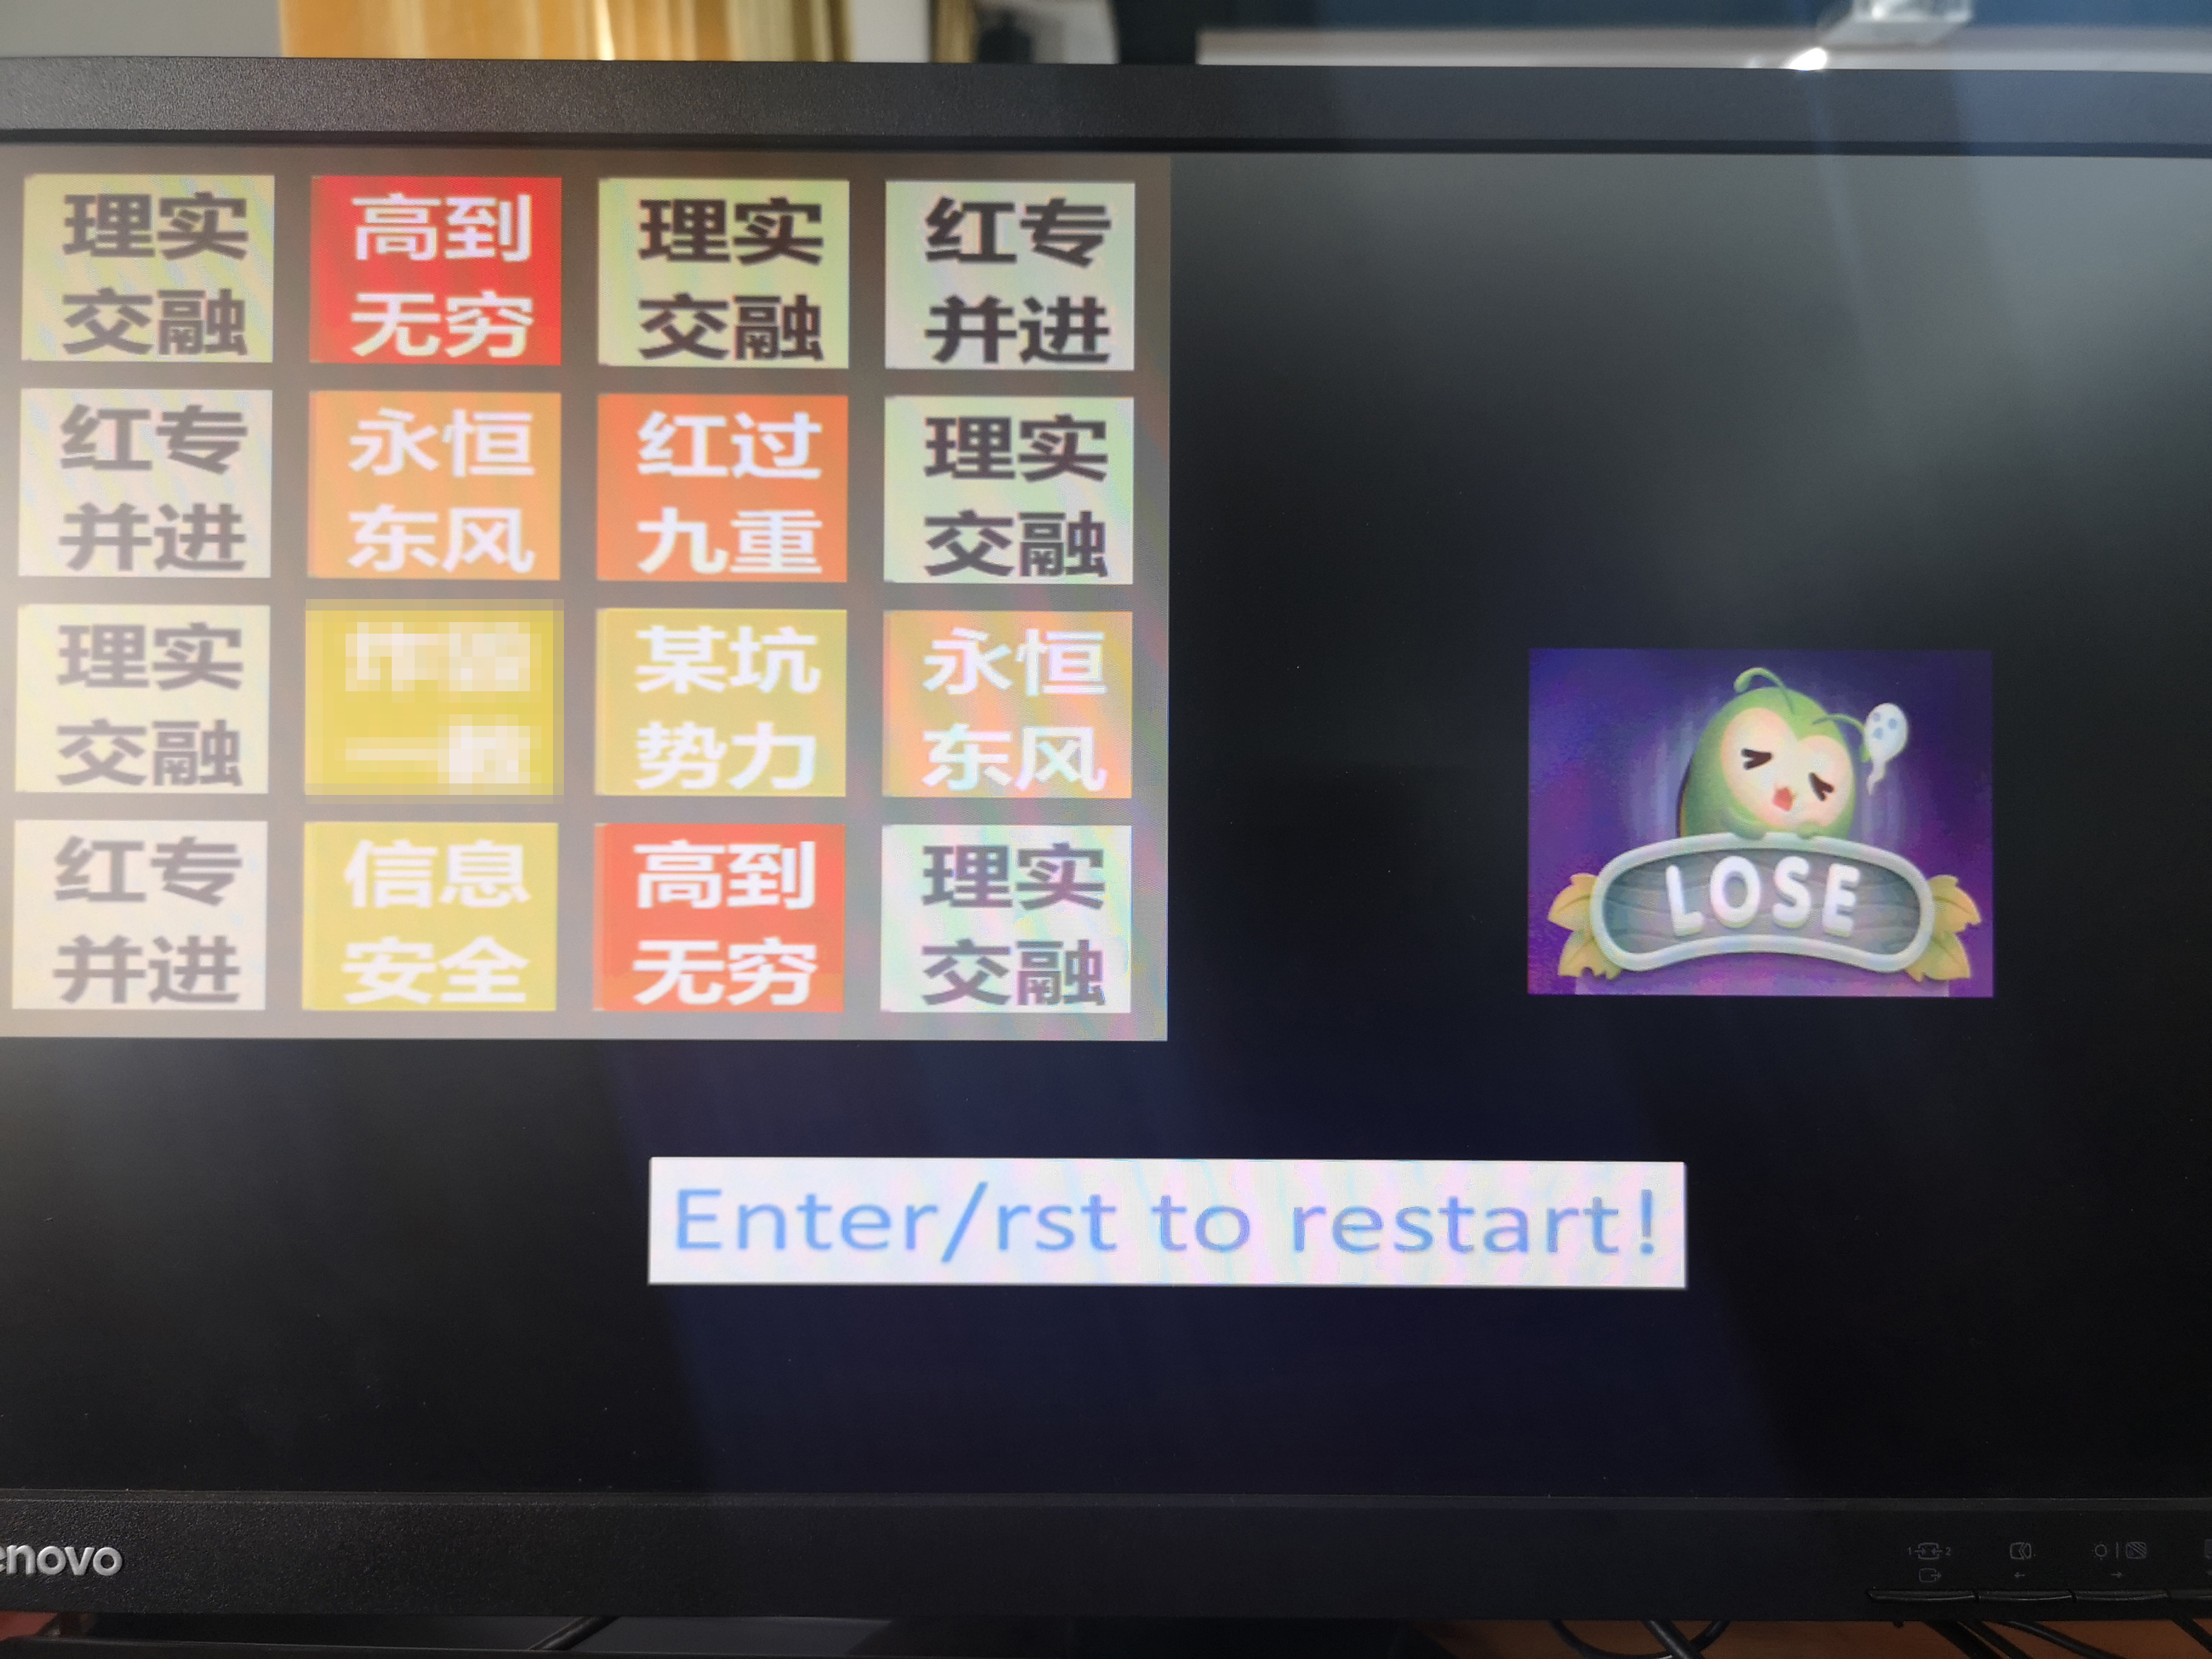
\includegraphics[scale=0.07]{fail.jpg}
		\caption{游戏失败界面}
		\label{fail}
	\end{figure}\par
	至于游戏成功的画面,由于我还不够强,没有成功过。不过和游戏失败时的是差不多的。\par

	
	\section{总结与思考}	
	本次实验中,由于时间较为紧迫,故量力而为选择了做一个小游戏"2048"。整个项目工程量比较大,需要综合前面学过的所有知识,甚至要再新学习例如VGA和PS2等这样的新接口。因此在整个过程中,我也踩了不少的坑。而正是这些坑,让我对于工程任务的完成有了更进一步的认识,使我的能力不断提升。此外在整个项目的实现过程中,我也深刻地体会到了模块化来使用硬件描述语言的方便和清晰,学会了各种各样的外设的使用。\par
	总而言之,本次项目实验确实让我得到比较大的提高,也让我对此产生更加深厚的兴趣。只可惜期末临近,时间紧迫,没能完成更加出色的项目,实在遗憾。好在所定目标也按时完成,给了自己一点欣慰的感觉。\par
	
	
	\subsection{本次实验的收获}
	收获特别大。学会了包括但不限于VGA,PS2等外设的使用,并能够用模块化的思想完成整个项目。\par
	
	\subsection{评价本次实验的难易程度}
	由于是大作业,实验难度不小。\par
	
	\subsection{评价本次实验的任务量}
	由于是大作业,任务量当然也很大。\par
	
	\subsection{为本次实验提供改进建议}
	在使用键盘外设的时候,由于没有合适的键盘,造成各种各样的问题。希望实验室能够购置合适的键盘。\par
	
	\newpage 
	\section{附录}
	\subsection{附录A.top模块代码}
	\begin{lstlisting}[language=Verilog]
	module FLXG(
		input clk,           // 输入时钟信号
		input PS2_CLK,
		input PS2_DATA,
		input rst,           // 输入复位信号
		input BTNL, BTNR, BTNU, BTND,
		output [3:0] red,    // 输出红色
		output [3:0] green,  // 输出绿色
		output [3:0] blue,   // 输出蓝色
		output hs,           // 水平同步信号
		output vs,            // 垂直同步信号
		output reg [15:0] LED,
		output [7:0] seg,
		output [7:0] AN
		);
	
	reg [63:0] Display_Num = 64'h0270024120201111;
	//reg [63:0] Display_Num = 64'h1212212112122121;
	wire [63:0] Display_Num_Right;
	wire [63:0] Display_Num_Left;
	wire [63:0] Display_Num_Up;
	wire [63:0] Display_Num_Down;
	wire ok_Left, ok_Right, ok_Down, ok_Up;
	
	reg [1:0] Global_Status = 0;
	parameter gaming = 0;
	parameter success = 1;
	parameter fail = 2;
	parameter target = 11;
	
	wire enter;
	wire [3:0] arrow_key;
	
	//总控制部分
	always @(negedge clk)
	begin
		if(rst || enter)
		begin
			Display_Num <= 64'h0000_0000_0000_0001;
			LED[15:4] <= 12'h000;
			LED[3:0] <= arrow_key;
		end
		else if(Global_Status == success)
		begin
			Display_Num <= Display_Num;
			LED[11:4] <= 8'hF0;
			LED[3:0] <= arrow_key;
		end
		else if(Global_Status == fail)
		begin
			Display_Num <= Display_Num;
			LED[11:4] <= 8'h0F;
			LED[3:0] <= arrow_key;
		end
		else if(Global_Status == gaming)
		begin
			if(ok_Up)
			begin
				Display_Num <= Display_Num_Up;
				LED[15] <= 1'b1;
				LED[3:0] <= arrow_key;
			end
			else if(ok_Down)
			begin
				Display_Num <= Display_Num_Down;
				LED[14] <= 1'b1;
				LED[3:0] <= arrow_key;
			end
			else if(ok_Left)
			begin
				Display_Num <= Display_Num_Left;
				LED[12] <= 1'b1;
				LED[3:0] <= arrow_key;
			end
			else if(ok_Right)
			begin
				Display_Num <= Display_Num_Right;
				LED[13] <= 1'b1;
				LED[3:0] <= arrow_key;
			end
			else
			begin
				Display_Num <= Display_Num;
				LED[15:4] = 12'h0000;
				LED[3:0] <= arrow_key;
			end 
		end
	end
	
	//VGA显示模块
	VGA VGA(.clk(clk), .rst(rst), .status(Global_Status), .Display_Num(Display_Num), .red(red), .green(green), .blue(blue), .hs(hs), .vs(vs));
	
	//PS2Receiver PS2Receiver(.clk(clk), .kclk(PS2_CLK), .kdata(PS2_DATA), .LED(arrow_key));
	Keyboard Keyboard(.clk(clk), .rst(rst), .ps2_clk(PS2_CLK), .ps2_data(PS2_DATA), .LED(arrow_key), .enter(enter));
	
	//上移模块
	Up_Move Up_Move(
		.rst(rst),
		.clk(clk),
		.Signal(BTNU),
		.key(arrow_key[0]),
		.input_state(Display_Num),
		.Display_Num(Display_Num_Up),
		.ok(ok_Up)
		);
	
	//下移模块
	Down_Move Down_Move(
		.rst(rst),
		.clk(clk),
		.Signal(BTND),
		.key(arrow_key[1]),
		.input_state(Display_Num),
		.Display_Num(Display_Num_Down),
		.ok(ok_Down)
		);
	
	//左移模块
	Left_Move Left_Move(
		.rst(rst),
		.clk(clk),
		.Signal(BTNL),
		.key(arrow_key[3]),
		.input_state(Display_Num),
		.Display_Num(Display_Num_Left),
		.ok(ok_Left)
		);
	
	//右移模块
	Right_Move Right_Move(
		.rst(rst),
		.clk(clk),
		.Signal(BTNR),
		.key(arrow_key[2]),
		.input_state(Display_Num),
		.Display_Num(Display_Num_Right),
		.ok(ok_Right)
		);
	
	//全局游戏状态判断器
	always @(posedge clk)
		begin
			if(Display_Num[3:0] == target || Display_Num[7:4] == target || Display_Num[11:8] == target || Display_Num[15:12] == target
			|| Display_Num[19:16] == target || Display_Num[23:20] == target || Display_Num[27:24] == target || Display_Num[31:28] == target
			|| Display_Num[35:32] == target || Display_Num[39:36] == target || Display_Num[43:40] == target || Display_Num[47:44] == target
			|| Display_Num[51:48] == target || Display_Num[55:52] == target || Display_Num[59:56] == target || Display_Num[63:60] == target)
		begin
			Global_Status <= success;
		end
			else if((Display_Num[3:0] != 4'h0 && Display_Num[7:4] != 4'h0 && Display_Num[11:8] != 4'h0 && Display_Num[15:12] != 4'h0
			&& Display_Num[19:16] != 4'h0 && Display_Num[23:20] != 4'h0 && Display_Num[27:24] != 4'h0 && Display_Num[31:28] != 4'h0
			&& Display_Num[35:32] != 4'h0 && Display_Num[39:36] != 4'h0 && Display_Num[43:40] != 4'h0 && Display_Num[47:44] != 4'h0
			&& Display_Num[51:48] != 4'h0 && Display_Num[55:52] != 4'h0 && Display_Num[59:56] != 4'h0 && Display_Num[63:60] != 4'h0)
			&&//前面判断都不是空,后面判断相邻都不同。
			(Display_Num[3:0] != Display_Num[7:4] && Display_Num[7:4] != Display_Num[11:8] && Display_Num[11:8] != Display_Num[15:12]
			&& Display_Num[19:16] != Display_Num[23:20] && Display_Num[23:20] != Display_Num[27:24] && Display_Num[27:24] != Display_Num[31:28]
			&& Display_Num[35:32] != Display_Num[39:36] && Display_Num[39:36] != Display_Num[43:40] && Display_Num[43:40] != Display_Num[47:44]
			&& Display_Num[51:48] != Display_Num[55:52] && Display_Num[55:52] != Display_Num[59:56] && Display_Num[59:56] != Display_Num[63:60]
			&& Display_Num[3:0] != Display_Num[19:16] && Display_Num[19:16] != Display_Num[35:32] && Display_Num[35:32] != Display_Num[51:48]
			&& Display_Num[7:4] != Display_Num[23:20] && Display_Num[23:20] != Display_Num[39:36] && Display_Num[39:36] != Display_Num[55:52]
			&& Display_Num[11:8] != Display_Num[27:24] && Display_Num[27:24] != Display_Num[43:40] && Display_Num[43:40] != Display_Num[59:56]
			&& Display_Num[15:12] != Display_Num[31:28] && Display_Num[31:28] != Display_Num[47:44] && Display_Num[47:44] != Display_Num[63:60]))
		begin
			Global_Status <= fail;
		end
		else
			Global_Status <= gaming;
	end
	
	reg [26:0] scores;
	wire [26:0] toAdd [15:0]; 
	Nixietube(.clk(clk), .rst(rst), .x(scores), .seg(seg), .AN(AN));
	dist_mem_gen_0 dist_mem_gen_0_0(.a(Display_Num[3:0]), .spo(toAdd[0]));
	dist_mem_gen_0 dist_mem_gen_0_1(.a(Display_Num[7:4]), .spo(toAdd[1]));
	dist_mem_gen_0 dist_mem_gen_0_2(.a(Display_Num[11:8]), .spo(toAdd[2]));
	dist_mem_gen_0 dist_mem_gen_0_3(.a(Display_Num[15:12]), .spo(toAdd[3]));
	dist_mem_gen_0 dist_mem_gen_0_4(.a(Display_Num[19:16]), .spo(toAdd[4]));
	dist_mem_gen_0 dist_mem_gen_0_5(.a(Display_Num[23:20]), .spo(toAdd[5]));
	dist_mem_gen_0 dist_mem_gen_0_6(.a(Display_Num[27:24]), .spo(toAdd[6]));
	dist_mem_gen_0 dist_mem_gen_0_7(.a(Display_Num[31:28]), .spo(toAdd[7]));
	dist_mem_gen_0 dist_mem_gen_0_8(.a(Display_Num[35:32]), .spo(toAdd[8]));
	dist_mem_gen_0 dist_mem_gen_0_9(.a(Display_Num[39:36]), .spo(toAdd[9]));
	dist_mem_gen_0 dist_mem_gen_0_10(.a(Display_Num[43:40]), .spo(toAdd[10]));
	dist_mem_gen_0 dist_mem_gen_0_11(.a(Display_Num[47:44]), .spo(toAdd[11]));
	dist_mem_gen_0 dist_mem_gen_0_12(.a(Display_Num[51:48]), .spo(toAdd[12]));
	dist_mem_gen_0 dist_mem_gen_0_13(.a(Display_Num[55:52]), .spo(toAdd[13]));
	dist_mem_gen_0 dist_mem_gen_0_14(.a(Display_Num[59:56]), .spo(toAdd[14]));
	dist_mem_gen_0 dist_mem_gen_0_15(.a(Display_Num[63:60]), .spo(toAdd[15]));
	
	
	always @(posedge clk)
	begin
		scores <= toAdd[0] + toAdd[1] + toAdd[2] + toAdd[3] + toAdd[4] + toAdd[5] + toAdd[6] + toAdd[7]
		+ toAdd[8] + toAdd[9] + toAdd[10] + toAdd[11] + toAdd[12] + toAdd[13] + toAdd[14] + toAdd[15];
	end
	endmodule
	\end{lstlisting}
	
	\subsection{附录B.VGA显示模块}
	\begin{lstlisting}[language=Verilog]
	module VGA( 
		input clk,                // 输入时钟信号
		input rst,                // 输入复位信号
		input [1:0] status,             // 游戏状态
		input [63:0] Display_Num,
		output reg [3:0] red,    // 输出红色
		output reg [3:0] green,  // 输出绿色
		output reg [3:0] blue,   // 输出蓝色
		output hs,               // 行同步信号
		output vs                // 场同步信号
		);
	
	// 分辨率为1024*768时行时序各个参数定义
	parameter H_SYNC_PULSE  = 136;
	parameter H_BACK_PORCH  = 160;
	parameter H_ACTIVE_TIME = 1024;
	parameter H_FRONT_PORCH = 24;
	parameter H_LINE_PERIOD = 1344;
	
	// 分辨率为1024*768时场时序各个参数定义         
	parameter V_SYNC_PULSE  = 6;
	parameter V_BACK_PORCH  = 29;
	parameter V_ACTIVE_TIME = 768;
	parameter V_FRONT_PORCH = 3;
	parameter V_LINE_PERIOD = 806;
	
	reg [11:0] h_cnt; // 行时序计数器
	reg [11:0] v_cnt; //场时序计数器
	wire clk_65M;
	
	wire active_flag; //激活标志,当这个信号为1时RGB的数据可以显示在屏幕上
	
	// generate a clock of 65MHZ
	wire locked;
		clk_wiz_65M clk_wiz_65M(
		.clk_in1(clk),
		.clk_out1(clk_65M),
		.reset(1'b0),
		.locked(locked));
	
	// 生成行时序
	always @(posedge clk_65M)
	begin
		if(h_cnt == H_LINE_PERIOD - 1'b1)
			h_cnt <= 12'd0;
		else
			h_cnt <= h_cnt + 1;
	end
	assign hs = (h_cnt < H_SYNC_PULSE) ? 1'b0 : 1'b1; 
	
	
	// 生成场时序
	always @(posedge clk_65M)
	begin
		if(v_cnt == V_LINE_PERIOD - 1'b1)
			v_cnt <= 12'd0;
		else if(h_cnt == H_LINE_PERIOD - 1'b1)
			v_cnt <= v_cnt + 1;
		else
			v_cnt <= v_cnt;
	end
	assign vs = (v_cnt < V_SYNC_PULSE) ? 1'b0 : 1'b1;
	
	// 当且仅当它处于有效区的时候,才被置为1
	assign active_flag =  
		(h_cnt >= (H_SYNC_PULSE + H_BACK_PORCH))  &&
		(h_cnt <= (H_SYNC_PULSE + H_BACK_PORCH + H_ACTIVE_TIME))  && 
		(v_cnt >= (V_SYNC_PULSE + V_BACK_PORCH))  &&
		(v_cnt <= (V_SYNC_PULSE + V_BACK_PORCH + V_ACTIVE_TIME));   
		
	parameter IMAGE_START_H = 668;
	parameter IMAGE_START_V = 284;
	parameter IMAGE_WIDTH = 200;
	parameter IMAGE_HEIGHT = 200;
	parameter IMAGE_PIX_NUM = 40000;
	
	reg [15:0] rom_addr;
	wire [11:0] rom_data;
	img_cwk img_cwk(.addra(rom_addr),.clka(clk_65M),.douta(rom_data),.ena(1'b1));
	
	reg [15:0] rom_addr_success;
	wire [11:0] rom_data_success;
	img_success img_success(.addra(rom_addr_success),.clka(clk_65M),.douta(rom_data_success),.ena(1'b1));
	
	reg [15:0] rom_addr_fail;
	wire [11:0] rom_data_fail;
	img_fail img_fail(.addra(rom_addr_fail),.clka(clk_65M),.douta(rom_data_fail),.ena(1'b1));
	
	parameter IMAGE_RST_START_H = 290;
	parameter IMAGE_RST_START_V = 580;
	parameter IMAGE_RST_WIDTH = 445;
	parameter IMAGE_RST_HEIGHT = 71;
	parameter IMAGE_RST_PIX_NUM = 31595;
	
	reg [14:0] rom_addr_rst;
	wire [11:0] rom_data_rst;
	img_rst img_rst(.addra(rom_addr_rst),.clka(clk_65M),.douta(rom_data_rst),.ena(1'b1));
	
	
	parameter BLOCK_WIDTH = 108;
	parameter BLOCK_PIX_NUM = 11664;
	
	parameter LAYOUT_WIDTH = 512;
	parameter LAYOUT_HEIGHT = 512;
	
	
	parameter FRAME_WIDTH = 16;
	parameter FRAME_START_H_0 = 0;
	parameter FRAME_START_H_1 = 124;
	parameter FRAME_START_H_2 = 248;
	parameter FRAME_START_H_3 = 372;
	parameter FRAME_START_H_4 = 496;
	parameter FRAME_START_V_0 = 0;
	parameter FRAME_START_V_1 = 124;
	parameter FRAME_START_V_2 = 248;
	parameter FRAME_START_V_3 = 372;
	parameter FRAME_START_V_4 = 496;
	
	parameter gaming = 0;
	parameter success = 1;
	parameter fail = 2;
	
	reg [3:0] block_index;
	reg [13:0] rom_addr_num [15:0];
	reg [13:0] rom_addr_num_input;
	wire [11:0] rom_data_num [10:0];
	
	// for flxg
	blk_mem_gen_num_none blk_mem_gen_num_none(.addra(rom_addr_num_input),.clka(clk_65M),.douta(rom_data_num[0]),.ena(1'b1));
	blk_mem_gen_2 blk_mem_gen_2(.addra(rom_addr_num_input),.clka(clk_65M),.douta(rom_data_num[1]),.ena(1'b1));
	blk_mem_gen_4 blk_mem_gen_4(.addra(rom_addr_num_input),.clka(clk_65M),.douta(rom_data_num[2]),.ena(1'b1));
	blk_mem_gen_8 blk_mem_gen_8(.addra(rom_addr_num_input),.clka(clk_65M),.douta(rom_data_num[3]),.ena(1'b1));
	blk_mem_gen_16 blk_mem_gen_16(.addra(rom_addr_num_input),.clka(clk_65M),.douta(rom_data_num[4]),.ena(1'b1));
	blk_mem_gen_32 blk_mem_gen_32(.addra(rom_addr_num_input),.clka(clk_65M),.douta(rom_data_num[5]),.ena(1'b1));
	blk_mem_gen_64 blk_mem_gen_64(.addra(rom_addr_num_input),.clka(clk_65M),.douta(rom_data_num[6]),.ena(1'b1));
	blk_mem_gen_128 blk_mem_gen_128(.addra(rom_addr_num_input),.clka(clk_65M),.douta(rom_data_num[7]),.ena(1'b1));
	blk_mem_gen_256 blk_mem_gen_256(.addra(rom_addr_num_input),.clka(clk_65M),.douta(rom_data_num[8]),.ena(1'b1));
	blk_mem_gen_512 blk_mem_gen_512(.addra(rom_addr_num_input),.clka(clk_65M),.douta(rom_data_num[9]),.ena(1'b1));
	blk_mem_gen_1024 blk_mem_gen_1024(.addra(rom_addr_num_input),.clka(clk_65M),.douta(rom_data_num[10]),.ena(1'b1));
	blk_mem_gen_2048 blk_mem_gen_2048(.addra(rom_addr_num_input),.clka(clk_65M),.douta(rom_data_num[11]),.ena(1'b1));
	
	always @(posedge clk_65M)
	begin
		if(active_flag) 
		begin
			if(h_cnt >= (H_SYNC_PULSE + H_BACK_PORCH + IMAGE_START_H)  &&
				h_cnt <= (H_SYNC_PULSE + H_BACK_PORCH + IMAGE_WIDTH-1'b1 + IMAGE_START_H)  && 
				v_cnt >= (V_SYNC_PULSE + V_BACK_PORCH + IMAGE_START_V)  &&
				v_cnt <= (V_SYNC_PULSE + V_BACK_PORCH + IMAGE_HEIGHT-1'b1 + IMAGE_START_V))
			begin
				if(status == gaming)
				begin
					rom_addr_fail <=  15'd0 ;
					rom_addr_success <=  15'd0 ;
					red <= rom_data[11:8]; // 红色分量
					green <= rom_data[7:4]; // 绿色分量
					blue <= rom_data[3:0]; // 蓝色分量
					if(rom_addr == IMAGE_PIX_NUM - 1'b1)
						rom_addr  <=  15'd0 ;
					else
						rom_addr  <=  rom_addr  +  1'b1;  
				end
				else if(status == fail)
				begin
					rom_addr <=  15'd0 ;
					rom_addr_success <=  15'd0 ;
					red <= rom_data_fail[11:8]; // 红色分量
					green <= rom_data_fail[7:4]; // 绿色分量
					blue <= rom_data_fail[3:0]; // 蓝色分量
					if(rom_addr_fail == IMAGE_PIX_NUM - 1'b1)
						rom_addr_fail  <=  15'd0 ;
					else
						rom_addr_fail  <=  rom_addr_fail  +  1'b1;  
				end
				else if(status == success)
				begin
					rom_addr <=  15'd0 ;
					rom_addr_fail <=  15'd0 ;
					red <= rom_data_success[11:8]; // 红色分量
					green <= rom_data_success[7:4]; // 绿色分量
					blue <= rom_data_success[3:0]; // 蓝色分量
					if(rom_addr_success == IMAGE_PIX_NUM - 1'b1)
						rom_addr_success  <=  15'd0 ;
					else
						rom_addr_success  <=  rom_addr_success  +  1'b1;  
				end
			end
			else if(h_cnt >= (H_SYNC_PULSE + H_BACK_PORCH + IMAGE_RST_START_H)  &&
				h_cnt <= (H_SYNC_PULSE + H_BACK_PORCH + IMAGE_RST_WIDTH-1'b1 + IMAGE_RST_START_H)  && 
				v_cnt >= (V_SYNC_PULSE + V_BACK_PORCH + IMAGE_RST_START_V)  &&
				v_cnt <= (V_SYNC_PULSE + V_BACK_PORCH + IMAGE_RST_HEIGHT-1'b1 + IMAGE_RST_START_V))
			begin
				red <= rom_data_rst[11:8]; // 红色分量
				green <= rom_data_rst[7:4]; // 绿色分量
				blue <= rom_data_rst[3:0]; // 蓝色分量
				if(rom_addr_rst == IMAGE_RST_PIX_NUM - 1'b1)
					rom_addr_rst  <=  14'd0 ;
				else
					rom_addr_rst  <=  rom_addr_rst  +  1'b1;  
			end
			else if(
				//否则如果在游戏界面范围内ss
				h_cnt >= (H_SYNC_PULSE + H_BACK_PORCH)  &&
				h_cnt <= (H_SYNC_PULSE + H_BACK_PORCH + LAYOUT_WIDTH-1'b1)  && 
				v_cnt >= (V_SYNC_PULSE + V_BACK_PORCH)  &&
				v_cnt <= (V_SYNC_PULSE + V_BACK_PORCH + LAYOUT_HEIGHT-1'b1))
			begin
				// 判断是不是在框的范围内
				if(
					((h_cnt >= (H_SYNC_PULSE + H_BACK_PORCH + FRAME_START_H_0) &&
					h_cnt <= (H_SYNC_PULSE + H_BACK_PORCH + FRAME_WIDTH-1'b1 + FRAME_START_H_0)) || 
					(h_cnt >= (H_SYNC_PULSE + H_BACK_PORCH + FRAME_START_H_1) &&
					h_cnt <= (H_SYNC_PULSE + H_BACK_PORCH + FRAME_WIDTH-1'b1 + FRAME_START_H_1)) ||
					(h_cnt >= (H_SYNC_PULSE + H_BACK_PORCH + FRAME_START_H_2) &&
					h_cnt <= (H_SYNC_PULSE + H_BACK_PORCH + FRAME_WIDTH-1'b1 + FRAME_START_H_2)) || 
					(h_cnt >= (H_SYNC_PULSE + H_BACK_PORCH + FRAME_START_H_3) &&
					h_cnt <= (H_SYNC_PULSE + H_BACK_PORCH + FRAME_WIDTH-1'b1 + FRAME_START_H_3)) || 
					(h_cnt >= (H_SYNC_PULSE + H_BACK_PORCH + FRAME_START_H_4) &&
					h_cnt <= (H_SYNC_PULSE + H_BACK_PORCH + FRAME_WIDTH-1'b1 + FRAME_START_H_4))) 
					|| 
					((v_cnt >= (V_SYNC_PULSE + V_BACK_PORCH + FRAME_START_V_0) &&
					v_cnt <= (V_SYNC_PULSE + V_BACK_PORCH + FRAME_WIDTH-1'b1 + FRAME_START_V_0)) ||
					(v_cnt >= (V_SYNC_PULSE + V_BACK_PORCH + FRAME_START_V_1) &&
					v_cnt <= (V_SYNC_PULSE + V_BACK_PORCH + FRAME_WIDTH-1'b1 + FRAME_START_V_1)) ||
					(v_cnt >= (V_SYNC_PULSE + V_BACK_PORCH + FRAME_START_V_2) &&
					v_cnt <= (V_SYNC_PULSE + V_BACK_PORCH + FRAME_WIDTH-1'b1 + FRAME_START_V_2)) ||
					(v_cnt >= (V_SYNC_PULSE + V_BACK_PORCH + FRAME_START_V_3) &&
					v_cnt <= (V_SYNC_PULSE + V_BACK_PORCH + FRAME_WIDTH-1'b1 + FRAME_START_V_3)) ||
					(v_cnt >= (V_SYNC_PULSE + V_BACK_PORCH + FRAME_START_V_4) &&
					v_cnt <= (V_SYNC_PULSE + V_BACK_PORCH + FRAME_WIDTH-1'b1 + FRAME_START_V_4))))
				begin
					red <= 4'd9;
					green <= 4'd8;
					blue <= 4'd7;
				end
				else
				begin
					//(0,0)块
					if(
						h_cnt >= (H_SYNC_PULSE + H_BACK_PORCH - BLOCK_WIDTH + FRAME_START_H_1) &&
						h_cnt <= (H_SYNC_PULSE + H_BACK_PORCH - 1'b1 + FRAME_START_H_1) && 
						v_cnt >= (V_SYNC_PULSE + V_BACK_PORCH - BLOCK_WIDTH + FRAME_START_V_1) &&
						v_cnt <= (V_SYNC_PULSE + V_BACK_PORCH - 1'b1 + FRAME_START_V_1))
					begin
						rom_addr_num_input <= rom_addr_num[0];
						{red, green, blue} <= rom_data_num[Display_Num[3:0]];
						if(rom_addr_num[0] == BLOCK_PIX_NUM - 1'b1) rom_addr_num[0] <=  13'd0;
						else rom_addr_num[0] <=  rom_addr_num[0] + 1'b1;
					end
					//(0,1)块
					else if(
						h_cnt >= (H_SYNC_PULSE + H_BACK_PORCH - BLOCK_WIDTH + FRAME_START_H_2) &&
						h_cnt <= (H_SYNC_PULSE + H_BACK_PORCH - 1'b1 + FRAME_START_H_2)  && 
						v_cnt >= (V_SYNC_PULSE + V_BACK_PORCH - BLOCK_WIDTH + FRAME_START_V_1) &&
						v_cnt <= (V_SYNC_PULSE + V_BACK_PORCH - 1'b1 + FRAME_START_V_1))
					begin
						rom_addr_num_input <= rom_addr_num[1];
						{red, green, blue} <= rom_data_num[Display_Num[7:4]];
						if(rom_addr_num[1] == BLOCK_PIX_NUM - 1'b1) rom_addr_num[1] <=  13'd0;
						else rom_addr_num[1] <=  rom_addr_num[1] + 1'b1;
					end
					//(0,2)块
					else if(
						h_cnt >= (H_SYNC_PULSE + H_BACK_PORCH - BLOCK_WIDTH + FRAME_START_H_3) &&
						h_cnt <= (H_SYNC_PULSE + H_BACK_PORCH - 1'b1 + FRAME_START_H_3)  && 
						v_cnt >= (V_SYNC_PULSE + V_BACK_PORCH - BLOCK_WIDTH + FRAME_START_V_1) &&
						v_cnt <= (V_SYNC_PULSE + V_BACK_PORCH - 1'b1 + FRAME_START_V_1))
					begin
						rom_addr_num_input <= rom_addr_num[2];
						{red, green, blue} <= rom_data_num[Display_Num[11:8]];
						if(rom_addr_num[2] == BLOCK_PIX_NUM - 1'b1) rom_addr_num[2] <=  13'd0;
						else rom_addr_num[2] <=  rom_addr_num[2] + 1'b1;
					end
					//(0,3)块
					else if(
						h_cnt >= (H_SYNC_PULSE + H_BACK_PORCH - BLOCK_WIDTH + FRAME_START_H_4) &&
						h_cnt <= (H_SYNC_PULSE + H_BACK_PORCH - 1'b1 + FRAME_START_H_4)  && 
						v_cnt >= (V_SYNC_PULSE + V_BACK_PORCH - BLOCK_WIDTH + FRAME_START_V_1) &&
						v_cnt <= (V_SYNC_PULSE + V_BACK_PORCH - 1'b1 + FRAME_START_V_1))
					begin
						rom_addr_num_input <= rom_addr_num[3];
						{red, green, blue} <= rom_data_num[Display_Num[15:12]];
						if(rom_addr_num[3] == BLOCK_PIX_NUM - 1'b1) rom_addr_num[3] <=  13'd0;
						else rom_addr_num[3] <=  rom_addr_num[3] + 1'b1;
					end
					//(1,0)块
					else if(
						h_cnt >= (H_SYNC_PULSE + H_BACK_PORCH - BLOCK_WIDTH + FRAME_START_H_1) &&
						h_cnt <= (H_SYNC_PULSE + H_BACK_PORCH - 1'b1 + FRAME_START_H_1) && 
						v_cnt >= (V_SYNC_PULSE + V_BACK_PORCH - BLOCK_WIDTH + FRAME_START_V_2) &&
						v_cnt <= (V_SYNC_PULSE + V_BACK_PORCH - 1'b1 + FRAME_START_V_2))
					begin
						rom_addr_num_input <= rom_addr_num[4];
						{red, green, blue} <= rom_data_num[Display_Num[19:16]];
						if(rom_addr_num[4] == BLOCK_PIX_NUM - 1'b1) rom_addr_num[4] <=  13'd0;
						else rom_addr_num[4] <=  rom_addr_num[4] + 1'b1;
					end
					//(1,1)块
					else if(
						h_cnt >= (H_SYNC_PULSE + H_BACK_PORCH - BLOCK_WIDTH + FRAME_START_H_2) &&
						h_cnt <= (H_SYNC_PULSE + H_BACK_PORCH - 1'b1 + FRAME_START_H_2)  && 
						v_cnt >= (V_SYNC_PULSE + V_BACK_PORCH - BLOCK_WIDTH + FRAME_START_V_2) &&
						v_cnt <= (V_SYNC_PULSE + V_BACK_PORCH - 1'b1 + FRAME_START_V_2))
					begin
						rom_addr_num_input <= rom_addr_num[5];
						{red, green, blue} <= rom_data_num[Display_Num[23:20]];
						if(rom_addr_num[5] == BLOCK_PIX_NUM - 1'b1) rom_addr_num[5] <=  13'd0;
						else rom_addr_num[5] <=  rom_addr_num[5] + 1'b1;
					end
					//(1,2)块
					else if(
						h_cnt >= (H_SYNC_PULSE + H_BACK_PORCH - BLOCK_WIDTH + FRAME_START_H_3) &&
						h_cnt <= (H_SYNC_PULSE + H_BACK_PORCH - 1'b1 + FRAME_START_H_3)  && 
						v_cnt >= (V_SYNC_PULSE + V_BACK_PORCH - BLOCK_WIDTH + FRAME_START_V_2) &&
						v_cnt <= (V_SYNC_PULSE + V_BACK_PORCH - 1'b1 + FRAME_START_V_2))
					begin
						rom_addr_num_input <= rom_addr_num[6];
						{red, green, blue} <= rom_data_num[Display_Num[27:24]];
						if(rom_addr_num[6] == BLOCK_PIX_NUM - 1'b1) rom_addr_num[6] <=  13'd0;
						else rom_addr_num[6] <=  rom_addr_num[6] + 1'b1;
					end
					//(1,3)块
					else if(
						h_cnt >= (H_SYNC_PULSE + H_BACK_PORCH - BLOCK_WIDTH + FRAME_START_H_4) &&
						h_cnt <= (H_SYNC_PULSE + H_BACK_PORCH - 1'b1 + FRAME_START_H_4)  && 
						v_cnt >= (V_SYNC_PULSE + V_BACK_PORCH - BLOCK_WIDTH + FRAME_START_V_2) &&
						v_cnt <= (V_SYNC_PULSE + V_BACK_PORCH - 1'b1 + FRAME_START_V_2))
					begin
						rom_addr_num_input <= rom_addr_num[7];
						{red, green, blue} <= rom_data_num[Display_Num[31:28]];
						if(rom_addr_num[7] == BLOCK_PIX_NUM - 1'b1) rom_addr_num[7] <=  13'd0;
						else rom_addr_num[7] <=  rom_addr_num[7] + 1'b1;
					end
					//(2,0)块
					else if(
						h_cnt >= (H_SYNC_PULSE + H_BACK_PORCH - BLOCK_WIDTH + FRAME_START_H_1) &&
						h_cnt <= (H_SYNC_PULSE + H_BACK_PORCH - 1'b1 + FRAME_START_H_1) && 
						v_cnt >= (V_SYNC_PULSE + V_BACK_PORCH - BLOCK_WIDTH + FRAME_START_V_3) &&
						v_cnt <= (V_SYNC_PULSE + V_BACK_PORCH - 1'b1 + FRAME_START_V_3))
					begin
						rom_addr_num_input <= rom_addr_num[8];
						{red, green, blue} <= rom_data_num[Display_Num[35:32]];
						if(rom_addr_num[8] == BLOCK_PIX_NUM - 1'b1) rom_addr_num[8] <=  13'd0;
						else rom_addr_num[8] <=  rom_addr_num[8] + 1'b1;
					end
					//(2,1)块
					else if(
						h_cnt >= (H_SYNC_PULSE + H_BACK_PORCH - BLOCK_WIDTH + FRAME_START_H_2) &&
						h_cnt <= (H_SYNC_PULSE + H_BACK_PORCH - 1'b1 + FRAME_START_H_2)  && 
						v_cnt >= (V_SYNC_PULSE + V_BACK_PORCH - BLOCK_WIDTH + FRAME_START_V_3) &&
						v_cnt <= (V_SYNC_PULSE + V_BACK_PORCH - 1'b1 + FRAME_START_V_3))
					begin
						rom_addr_num_input <= rom_addr_num[9];
						{red, green, blue} <= rom_data_num[Display_Num[39:36]];
						if(rom_addr_num[9] == BLOCK_PIX_NUM - 1'b1) rom_addr_num[9] <=  13'd0;
						else rom_addr_num[9] <=  rom_addr_num[9] + 1'b1;
					end
					//(2,2)块
					else if(
						h_cnt >= (H_SYNC_PULSE + H_BACK_PORCH - BLOCK_WIDTH + FRAME_START_H_3) &&
						h_cnt <= (H_SYNC_PULSE + H_BACK_PORCH - 1'b1 + FRAME_START_H_3)  && 
						v_cnt >= (V_SYNC_PULSE + V_BACK_PORCH - BLOCK_WIDTH + FRAME_START_V_3) &&
						v_cnt <= (V_SYNC_PULSE + V_BACK_PORCH - 1'b1 + FRAME_START_V_3))
					begin
						rom_addr_num_input <= rom_addr_num[10];
						{red, green, blue} <= rom_data_num[Display_Num[43:40]];
						if(rom_addr_num[10] == BLOCK_PIX_NUM - 1'b1) rom_addr_num[10] <=  13'd0;
						else rom_addr_num[10] <=  rom_addr_num[10] + 1'b1;
					end
					//(2,3)块
					else if(
						h_cnt >= (H_SYNC_PULSE + H_BACK_PORCH - BLOCK_WIDTH + FRAME_START_H_4) &&
						h_cnt <= (H_SYNC_PULSE + H_BACK_PORCH - 1'b1 + FRAME_START_H_4)  && 
						v_cnt >= (V_SYNC_PULSE + V_BACK_PORCH - BLOCK_WIDTH + FRAME_START_V_3) &&
						v_cnt <= (V_SYNC_PULSE + V_BACK_PORCH - 1'b1 + FRAME_START_V_3))
					begin
						rom_addr_num_input <= rom_addr_num[11];
						{red, green, blue} <= rom_data_num[Display_Num[47:44]];
						if(rom_addr_num[11] == BLOCK_PIX_NUM - 1'b1) rom_addr_num[11] <=  13'd0;
						else rom_addr_num[11] <=  rom_addr_num[11] + 1'b1;
					end
					//(3,0)块
					else if(
						h_cnt >= (H_SYNC_PULSE + H_BACK_PORCH - BLOCK_WIDTH + FRAME_START_H_1) &&
						h_cnt <= (H_SYNC_PULSE + H_BACK_PORCH - 1'b1 + FRAME_START_H_1) && 
						v_cnt >= (V_SYNC_PULSE + V_BACK_PORCH - BLOCK_WIDTH + FRAME_START_V_4) &&
						v_cnt <= (V_SYNC_PULSE + V_BACK_PORCH - 1'b1 + FRAME_START_V_4))
					begin
						rom_addr_num_input <= rom_addr_num[12];
						{red, green, blue} <= rom_data_num[Display_Num[51:48]];
						if(rom_addr_num[12] == BLOCK_PIX_NUM - 1'b1) rom_addr_num[12] <=  13'd0;
						else rom_addr_num[12] <=  rom_addr_num[12] + 1'b1;
					end
					//(3,1)块
					else if(
						h_cnt >= (H_SYNC_PULSE + H_BACK_PORCH - BLOCK_WIDTH + FRAME_START_H_2) &&
						h_cnt <= (H_SYNC_PULSE + H_BACK_PORCH - 1'b1 + FRAME_START_H_2)  && 
						v_cnt >= (V_SYNC_PULSE + V_BACK_PORCH - BLOCK_WIDTH + FRAME_START_V_4) &&
						v_cnt <= (V_SYNC_PULSE + V_BACK_PORCH - 1'b1 + FRAME_START_V_4))
					begin
						rom_addr_num_input <= rom_addr_num[13];
						{red, green, blue} <= rom_data_num[Display_Num[55:52]];
						if(rom_addr_num[13] == BLOCK_PIX_NUM - 1'b1) rom_addr_num[13] <=  13'd0;
						else rom_addr_num[13] <=  rom_addr_num[13] + 1'b1;
					end
					//(3,2)块
					else if(
						h_cnt >= (H_SYNC_PULSE + H_BACK_PORCH - BLOCK_WIDTH + FRAME_START_H_3) &&
						h_cnt <= (H_SYNC_PULSE + H_BACK_PORCH - 1'b1 + FRAME_START_H_3)  && 
						v_cnt >= (V_SYNC_PULSE + V_BACK_PORCH - BLOCK_WIDTH + FRAME_START_V_4) &&
						v_cnt <= (V_SYNC_PULSE + V_BACK_PORCH - 1'b1 + FRAME_START_V_4))
					begin
						rom_addr_num_input <= rom_addr_num[14];
						{red, green, blue} <= rom_data_num[Display_Num[59:56]];
						if(rom_addr_num[14] == BLOCK_PIX_NUM - 1'b1) rom_addr_num[14] <=  13'd0;
						else rom_addr_num[14] <=  rom_addr_num[14] + 1'b1;
					end
					//(3,3)块
					else if(
						h_cnt >= (H_SYNC_PULSE + H_BACK_PORCH - BLOCK_WIDTH + FRAME_START_H_4) &&
						h_cnt <= (H_SYNC_PULSE + H_BACK_PORCH - 1'b1 + FRAME_START_H_4)  && 
						v_cnt >= (V_SYNC_PULSE + V_BACK_PORCH - BLOCK_WIDTH + FRAME_START_V_4) &&
						v_cnt <= (V_SYNC_PULSE + V_BACK_PORCH - 1'b1 + FRAME_START_V_4))
					begin
						rom_addr_num_input <= rom_addr_num[15];
						{red, green, blue} <= rom_data_num[Display_Num[63:60]];
						if(rom_addr_num[15] == BLOCK_PIX_NUM - 1'b1) rom_addr_num[15] <=  13'd0;
						else rom_addr_num[15] <=  rom_addr_num[15] + 1'b1;
					end
					else
					begin
						red <= 4'd12; green <= 4'd11; blue <= 4'd10;
					end
				end
			end
			else
			begin
				red <= 4'd0; green <= 4'd0; blue <= 4'd0; rom_addr <= rom_addr;
			end
		end  
		else
		begin
			red <= 4'd0;
			green <= 4'd0;
			blue <= 4'd0;
			rom_addr <= rom_addr;
		end           
	end
	
	endmodule
	\end{lstlisting}
	
	\subsection{附录C.向上平移模块代码(其他方向的就不再展示了)}
	\begin{lstlisting}[language=Verilog]
	module Up_Move(
		input rst,
		input clk,
		input Signal,
		input key,
		input [63:0] input_state,
		output reg [63:0] Display_Num,
		output ok
		);
	
	reg flag = 0;
	reg [63:0] last_state;
	
	//取移动信号边沿
	integer Signal_counter;
	integer key_counter;
	reg Signal_0, Signal_1, Signal_2, Signal_3;
	reg key_0, key_1, key_2, key_3;
	wire Signal_Redge, key_Redge;
	always @(posedge clk) key_1 <= key_0;
	always @(posedge clk) key_2 <= key_1;
	assign key_Redge = key_1 & ~key_2;
	always @(posedge clk) key_3 <= key_2;
	always @(posedge clk) Signal_1 <= Signal_0;
	always @(posedge clk) Signal_2 <= Signal_1;
	assign Signal_Redge = Signal_1 & ~Signal_2;
	always @(posedge clk) Signal_3 <= Signal_2;
	assign ok = (~Signal_1 & Signal_2) | (key_3);
	
	//去抖动
	always @(posedge clk)
	begin
		if(Signal)
		begin
			if(Signal_counter >= 100000)
			begin
				Signal_counter <= 100000;        
				Signal_0 <= 1;
			end
			else
				Signal_counter <= Signal_counter + 1;
		end
		else
		begin
			Signal_counter <= 0;
			Signal_0 <= 0;
		end
	end
	
	//去抖动
	always @(posedge clk)
	begin
		if(key)
		begin
			if(key_counter >= 100000)
			begin
				key_counter <= 100000;        
				key_0 <= 1;
			end
			else
				key_counter <= key_counter + 1;
		end
		else
		begin
			key_counter <= 0;
			key_0 <= 0;
		end
	end
	
	reg [1:0] random_counter = 0;
	always @(posedge clk)
	begin
		random_counter <= random_counter + 2'h1;
	end
	
	
	always @(posedge clk)
	begin
		if(rst)
		begin
			flag = 0;
			last_state = input_state;
			Display_Num = input_state;
		end
		else if(Signal_Redge || key_Redge) //如果有操作信号
		begin
			last_state = input_state;
			//对第一列的处理开始
			//首先补齐空缺位置
			if(last_state[3:0] == 4'h0) begin last_state[3:0] = last_state[19:16]; last_state[19:16] = last_state[35:32]; last_state[35:32] = last_state[51:48]; last_state[51:48] = 0; end
			if(last_state[3:0] == 4'h0) begin last_state[3:0] = last_state[19:16]; last_state[19:16] = last_state[35:32]; last_state[35:32] = last_state[51:48]; last_state[51:48] = 0; end
			if(last_state[3:0] == 4'h0) begin last_state[3:0] = last_state[19:16]; last_state[19:16] = last_state[35:32]; last_state[35:32] = last_state[51:48]; last_state[51:48] = 0; end
			if(last_state[3:0] == 4'h0) begin last_state[3:0] = last_state[19:16]; last_state[19:16] = last_state[35:32]; last_state[35:32] = last_state[51:48]; last_state[51:48] = 0; end
			if(last_state[19:16] == 4'h0) begin last_state[19:16] = last_state[35:32]; last_state[35:32] = last_state[51:48]; last_state[51:48] = 0; end
			if(last_state[19:16] == 4'h0) begin last_state[19:16] = last_state[35:32]; last_state[35:32] = last_state[51:48]; last_state[51:48] = 0; end
			if(last_state[19:16] == 4'h0) begin last_state[19:16] = last_state[35:32]; last_state[35:32] = last_state[51:48]; last_state[51:48] = 0; end
			if(last_state[35:32] == 4'h0) begin last_state[35:32] = last_state[51:48]; last_state[51:48] = 0; end
			if(last_state[35:32] == 4'h0) begin last_state[35:32] = last_state[51:48]; last_state[51:48] = 0; end
			//然后对方块的合并做处理
			if(last_state[3:0] == last_state[19:16] && last_state[35:32] == last_state[51:48]
			&& last_state[51:48] != 0 && last_state[19:16] != 0)
			begin
				last_state[3:0] = last_state[3:0] + 4'h1;
				last_state[19:16] = last_state[19:16] + 4'h1;
				last_state[35:32] = 4'h0; last_state[51:48] = 4'h0;
			end
			else if(last_state[3:0] == last_state[19:16] && last_state[19:16] != 0)
			begin
				last_state[3:0] = last_state[3:0] + 4'h1;
				last_state[19:16] = last_state[35:32];
				last_state[35:32] = last_state[51:48]; 
				last_state[51:48] = 4'h0;
			end
			else if(last_state[19:16] == last_state[35:32] && last_state[19:16] != 0)
			begin
				last_state[19:16] = last_state[19:16] + 4'h1;
				last_state[35:32] = last_state[51:48];
				last_state[51:48] = 4'h0;
			end
			else if(last_state[35:32] == last_state[51:48] && last_state[51:48] != 0)
			begin
				last_state[35:32] = last_state[35:32] + 4'h1; 
				last_state[51:48] = 4'h0;
			end
			//对第一列的处理结束
			
			//对第二列的处理开始
			if(last_state[7:4] == 4'h0) begin last_state[7:4] = last_state[23:20]; last_state[23:20] = last_state[39:36]; last_state[39:36] = last_state[55:52]; last_state[55:52] = 0; end
			if(last_state[7:4] == 4'h0) begin last_state[7:4] = last_state[23:20]; last_state[23:20] = last_state[39:36]; last_state[39:36] = last_state[55:52]; last_state[55:52] = 0; end
			if(last_state[7:4] == 4'h0) begin last_state[7:4] = last_state[23:20]; last_state[23:20] = last_state[39:36]; last_state[39:36] = last_state[55:52]; last_state[55:52] = 0; end
			if(last_state[7:4] == 4'h0) begin last_state[7:4] = last_state[23:20]; last_state[23:20] = last_state[39:36]; last_state[39:36] = last_state[55:52]; last_state[55:52] = 0; end
			if(last_state[23:20] == 4'h0) begin last_state[23:20] = last_state[39:36]; last_state[39:36] = last_state[55:52]; last_state[55:52] = 0; end
			if(last_state[23:20] == 4'h0) begin last_state[23:20] = last_state[39:36]; last_state[39:36] = last_state[55:52]; last_state[55:52] = 0; end
			if(last_state[23:20] == 4'h0) begin last_state[23:20] = last_state[39:36]; last_state[39:36] = last_state[55:52]; last_state[55:52] = 0; end
			if(last_state[39:36] == 4'h0) begin last_state[39:36] = last_state[55:52]; last_state[55:52] = 0; end
			if(last_state[39:36] == 4'h0) begin last_state[39:36] = last_state[55:52]; last_state[55:52] = 0; end
			//然后对方块的合并做处理
			if(last_state[7:4] == last_state[23:20] && last_state[39:36] == last_state[55:52]
			&& last_state[55:52] != 0 && last_state[23:20] != 0)
			begin
				last_state[7:4] = last_state[7:4] + 4'h1;
				last_state[23:20] = last_state[23:20] + 4'h1;
				last_state[39:36] = 4'h0; last_state[55:52] = 4'h0;
			end
			else if(last_state[7:4] == last_state[23:20] && last_state[23:20] != 0)
			begin
				last_state[7:4] = last_state[7:4] + 4'h1;
				last_state[23:20] = last_state[39:36];
				last_state[39:36] = last_state[55:52]; 
				last_state[55:52] = 4'h0;
			end
			else if(last_state[23:20] == last_state[39:36] && last_state[23:20] != 0)
			begin
				last_state[23:20] = last_state[23:20] + 4'h1;
				last_state[39:36] = last_state[55:52];
				last_state[55:52] = 4'h0;
			end
			else if(last_state[39:36] == last_state[55:52] && last_state[55:52] != 0)
			begin
				last_state[39:36] = last_state[39:36] + 4'h1; 
				last_state[55:52] = 4'h0;
			end
			//对第二列的处理结束
			
			//对第三列的处理开始
			if(last_state[11:8] == 4'h0) begin last_state[11:8] = last_state[27:24]; last_state[27:24] = last_state[43:40]; last_state[43:40] = last_state[59:56]; last_state[59:56] = 0; end
			if(last_state[11:8] == 4'h0) begin last_state[11:8] = last_state[27:24]; last_state[27:24] = last_state[43:40]; last_state[43:40] = last_state[59:56]; last_state[59:56] = 0; end
			if(last_state[11:8] == 4'h0) begin last_state[11:8] = last_state[27:24]; last_state[27:24] = last_state[43:40]; last_state[43:40] = last_state[59:56]; last_state[59:56] = 0; end
			if(last_state[11:8] == 4'h0) begin last_state[11:8] = last_state[27:24]; last_state[27:24] = last_state[43:40]; last_state[43:40] = last_state[59:56]; last_state[59:56] = 0; end
			if(last_state[27:24] == 4'h0) begin last_state[27:24] = last_state[43:40]; last_state[43:40] = last_state[59:56]; last_state[59:56] = 0; end
			if(last_state[27:24] == 4'h0) begin last_state[27:24] = last_state[43:40]; last_state[43:40] = last_state[59:56]; last_state[59:56] = 0; end
			if(last_state[27:24] == 4'h0) begin last_state[27:24] = last_state[43:40]; last_state[43:40] = last_state[59:56]; last_state[59:56] = 0; end
			if(last_state[43:40] == 4'h0) begin last_state[43:40] = last_state[59:56]; last_state[59:56] = 0; end
			if(last_state[43:40] == 4'h0) begin last_state[43:40] = last_state[59:56]; last_state[59:56] = 0; end
			//然后对方块的合并做处理
			if(last_state[11:8] == last_state[27:24] && last_state[43:40] == last_state[59:56]
			&& last_state[59:56] != 0 && last_state[27:24] != 0)
			begin
				last_state[11:8] = last_state[11:8] + 4'h1;
				last_state[27:24] = last_state[27:24] + 4'h1;
				last_state[43:40] = 4'h0; last_state[59:56] = 4'h0;
			end
			else if(last_state[11:8] == last_state[27:24] && last_state[27:24] != 0)
			begin
				last_state[11:8] = last_state[11:8] + 4'h1;
				last_state[27:24] = last_state[43:40];
				last_state[43:40] = last_state[59:56]; 
				last_state[59:56] = 4'h0;
			end
			else if(last_state[27:24] == last_state[43:40] && last_state[27:24] != 0)
			begin
				last_state[27:24] = last_state[27:24] + 4'h1;
				last_state[43:40] = last_state[59:56];
				last_state[59:56] = 4'h0;
			end
			else if(last_state[43:40] == last_state[59:56] && last_state[59:56] != 0)
			begin
				last_state[43:40] = last_state[43:40] + 4'h1; 
				last_state[59:56] = 4'h0;
			end
			//对第三列的处理结束
			
			//对第四列的处理开始
			if(last_state[15:12] == 4'h0) begin last_state[15:12] = last_state[31:28]; last_state[31:28] = last_state[47:44]; last_state[47:44] = last_state[63:60]; last_state[63:60] = 0; end
			if(last_state[15:12] == 4'h0) begin last_state[15:12] = last_state[31:28]; last_state[31:28] = last_state[47:44]; last_state[47:44] = last_state[63:60]; last_state[63:60] = 0; end
			if(last_state[15:12] == 4'h0) begin last_state[15:12] = last_state[31:28]; last_state[31:28] = last_state[47:44]; last_state[47:44] = last_state[63:60]; last_state[63:60] = 0; end
			if(last_state[15:12] == 4'h0) begin last_state[15:12] = last_state[31:28]; last_state[31:28] = last_state[47:44]; last_state[47:44] = last_state[63:60]; last_state[63:60] = 0; end
			if(last_state[31:28] == 4'h0) begin last_state[31:28] = last_state[47:44]; last_state[47:44] = last_state[63:60]; last_state[63:60] = 0; end
			if(last_state[31:28] == 4'h0) begin last_state[31:28] = last_state[47:44]; last_state[47:44] = last_state[63:60]; last_state[63:60] = 0; end
			if(last_state[31:28] == 4'h0) begin last_state[31:28] = last_state[47:44]; last_state[47:44] = last_state[63:60]; last_state[63:60] = 0; end
			if(last_state[47:44] == 4'h0) begin last_state[47:44] = last_state[63:60]; last_state[63:60] = 0; end
			if(last_state[47:44] == 4'h0) begin last_state[47:44] = last_state[63:60]; last_state[63:60] = 0; end
			//然后对方块的合并做处理
			if(last_state[15:12] == last_state[31:28] && last_state[47:44] == last_state[63:60]
			&& last_state[63:60] != 0 && last_state[31:28] != 0)
			begin
				last_state[15:12] = last_state[15:12] + 4'h1;
				last_state[31:28] = last_state[31:28] + 4'h1;
				last_state[47:44] = 4'h0; last_state[63:60] = 4'h0;
			end
			else if(last_state[15:12] == last_state[31:28] && last_state[31:28] != 0)
			begin
				last_state[15:12] = last_state[15:12] + 4'h1;
				last_state[31:28] = last_state[47:44];
				last_state[47:44] = last_state[63:60]; 
				last_state[63:60] = 4'h0;
			end
			else if(last_state[31:28] == last_state[47:44] && last_state[31:28] != 0)
			begin
				last_state[31:28] = last_state[31:28] + 4'h1;
				last_state[47:44] = last_state[63:60];
				last_state[63:60] = 4'h0;
			end
			else if(last_state[47:44] == last_state[63:60] && last_state[63:60] != 0)
			begin
				last_state[47:44] = last_state[47:44] + 4'h1; 
				last_state[63:60] = 4'h0;
			end
			//对第四列的处理结束
			
			//根据随机计数器random_counter新生成一个方块2,开始
			if(last_state != input_state)
			begin
				if(random_counter == 2'h0) 
				begin
					if(last_state[51:48] == 4'h0) last_state[51:48] = 4'h1;
					else if(last_state[55:52] == 4'h0) last_state[55:52] = 4'h1;
					else if(last_state[59:56] == 4'h0) last_state[59:56] = 4'h1;
					else if(last_state[63:60] == 4'h0) last_state[63:60] = 4'h1;
					else last_state = last_state;
				end
				else if(random_counter == 2'h1) 
				begin
					if(last_state[55:52] == 4'h0) last_state[55:52] = 4'h1;
					else if(last_state[59:56] == 4'h0) last_state[59:56] = 4'h1;
					else if(last_state[63:60] == 4'h0) last_state[63:60] = 4'h1;
					else if(last_state[51:48] == 4'h0) last_state[51:48] = 4'h1;
					else last_state = last_state;
				end
				else if(random_counter == 2'h2) 
				begin
					if(last_state[59:56] == 4'h0) last_state[59:56] = 4'h1;
					else if(last_state[63:60] == 4'h0) last_state[63:60] = 4'h1;
					else if(last_state[51:48] == 4'h0) last_state[51:48] = 4'h1;
					else if(last_state[55:52] == 4'h0) last_state[55:52] = 4'h1;
					else last_state = last_state;
				end
				else if(random_counter == 2'h3) 
				begin
					if(last_state[63:60] == 4'h0) last_state[63:60] = 4'h1;
					else if(last_state[51:48] == 4'h0) last_state[51:48] = 4'h1;
					else if(last_state[55:52] == 4'h0) last_state[55:52] = 4'h1;
					else if(last_state[59:56] == 4'h0) last_state[59:56] = 4'h1;
					else last_state = last_state;
				end
				else last_state = last_state;
			end
			else last_state = last_state;
			//根据随机计数器random_counter新生成一个方块2,结束
			
			flag = 1;
			Display_Num = last_state;
		end
	else
	begin
		if((Signal_0 && ~Signal_3) || (key_0 && ~key_3))
			Display_Num = input_state;
		else if(flag == 1)
			Display_Num = last_state;
		else
			Display_Num = input_state;
		end
	end
	
	
	endmodule
	\end{lstlisting}
	
	\subsection{附录D.键盘输入模块}
	\begin{lstlisting}[language=Verilog]
	module Keyboard(
		input clk,  //时钟信号
		input rst,  //复位信号
		input ps2_clk,  //PS2时钟信号
		input ps2_data, //PS2数据信号
		output reg	[3:0] LED,   //方向键按下信号
		output reg enter    //回车键按下信号
		);
	reg ps2_clk_r1,ps2_clk_r2;
	wire ps2_clk_neg;
	reg [3:0] ps2_clk_cnt;
	reg [15:0] key;
	
	always@(posedge clk or posedge rst) 
	begin
		if(rst) 
			ps2_clk_r1	<= 1'b1; 
		else 
			ps2_clk_r1	<= ps2_clk;
	end
	
	always@(posedge clk or posedge rst) 
	begin
		if(rst) 
			ps2_clk_r2	<= 1'b1;
		else 
			ps2_clk_r2	<= ps2_clk_r1;
	end
	
	assign ps2_clk_neg = (ps2_clk_r1==1'b0)&&(ps2_clk_r2==1'b1);
	
	always@(posedge clk or posedge rst) 
	begin
		if(rst) 
			ps2_clk_cnt <= 4'd0;
		else if(ps2_clk_neg)
		begin
			if(ps2_clk_cnt>=4'd10) 
				ps2_clk_cnt <= 4'd0;
			else 
				ps2_clk_cnt <= ps2_clk_cnt + 4'd1;
		end
	end
	
	always@(posedge clk or posedge rst) 
	begin
		if(rst)
			key <= 16'hFFFF;
		else if(ps2_clk_neg) //由PS2时钟信号确认工作状态
		begin
			//如果输入对应的8个数据位,则存入寄存器key中
			if((ps2_clk_cnt>=1)&&(ps2_clk_cnt<=8)) 
				key <= {ps2_data,key[15:1]};   
			else //否则key保持不变
				key <= key;
		end
	end
	
	always @(*)
	begin
		if(key[15:0] == 16'b0111010111110000)
		begin
			LED <= 4'b0001;
			enter <= 1'b0;
		end
		else if(key[15:0] == 16'b0111001011110000)
		begin
			LED <= 4'b0010;
			enter <= 1'b0;
		end
		else if(key[15:0] == 16'b0111010011110000)
		begin
			LED <= 4'b0100;
			enter <= 1'b0;
		end
		else if(key[15:0] == 16'b0110101111110000)
		begin
			LED <= 4'b1000;
			enter <= 1'b0;
		end
		else if(key[15:0] == 16'b0101101011110000)
		begin
			LED <= 4'b0000;
			enter <= 1'b1;
		end
		else
		begin
			LED <= 0000;
			enter <= 0;
		end
	end
	
	endmodule
	\end{lstlisting}
	
	\subsection{附录E.数码管模块}
	\begin{lstlisting}[language=Verilog]
	module Nixietube(
		input clk, rst, //时钟信号,复位信号
		input [26:0] x, //输入二进制数
		output reg [7:0] seg,   //输出数码管的显示
		output reg [7:0] AN     //输出数码管的选择
		);
	
	reg [31:0] counter;
	reg [58:0] dec;
	reg [3:0] dec_4;
	reg [2:0] stage;
	
	initial
	begin 
		AN <= 8'b1111_1110;
		counter <= 0;
		dec <= 0;
		dec_4 <= 0;
		stage <= 0;
	end
	
	// counter 计数
	always @(posedge clk or posedge rst)
	begin
		if(rst)
			counter <= 0;
		else if(counter == 32'd200000)
			counter <= 0;
		else
			counter <= counter + 1;
	end
	
	// 输出的dec_4的改变
	always @(posedge clk or posedge rst)
	begin
		if(rst)
		begin
			dec_4 <= dec[30:27];
			AN <= 8'b1111_1110;
			stage <= 0;
		end
		else
		begin
			if(counter == 32'd100000)
				stage = stage + 1;
			begin
			case(stage)
				3'b000: begin dec_4 <= dec[30:27]; AN <= 8'b1111_1110; end
				3'b001: begin dec_4 <= dec[34:31]; AN <= 8'b1111_1101; end
				3'b010: begin dec_4 <= dec[38:35]; AN = 8'b1111_1011; end
				3'b011: begin dec_4 <= dec[42:39]; AN = 8'b1111_0111; end
				3'b100: begin dec_4 <= dec[46:43]; AN <= 8'b1110_1111; end
				3'b101: begin dec_4 <= dec[50:47]; AN <= 8'b1101_1111; end
				3'b110: begin dec_4 <= dec[54:51]; AN <= 8'b1011_1111; end
				3'b111: begin dec_4 <= dec[58:55]; AN <= 8'b0111_1111; end
				default: begin dec_4 <= 4'bxxxx; AN <= 8'b1111_1110; end
			endcase
			end
		end
	end
	
	// 计算dec
	always @(posedge clk or posedge rst)
	begin
		if(rst)
			dec = 0;
		else 
		begin
			if(counter == 32'd100000)
			begin
				dec = 0;
				dec[26:0] = x;
				repeat(27)
				begin
					if(dec[58:55] >= 5 || dec[54:51] >= 5 || dec[50:47] >= 5 || dec[46:43] >= 5 || dec[42:39] >= 5 || dec[38:35] >= 5 || dec[34:31] >= 5 || dec[30:27] >= 5)
					begin
						if(dec[58:55] >= 5) dec[58:55] = dec[58:55] + 3;
						if(dec[54:51] >= 5) dec[54:51] = dec[54:51] + 3;
						if(dec[50:47] >= 5) dec[50:47] = dec[50:47] + 3;
						if(dec[46:43] >= 5) dec[46:43] = dec[46:43] + 3;
						if(dec[42:39] >= 5) dec[42:39] = dec[42:39] + 3;
						if(dec[38:35] >= 5) dec[38:35] = dec[38:35] + 3;
						if(dec[34:31] >= 5) dec[34:31] = dec[34:31] + 3;
						if(dec[30:27] >= 5) dec[30:27] = dec[30:27] + 3;
					end
					dec = dec << 1;
				end
			end
		end
	end
	
	// 根据dec_4修改seg
	always@(*)
	begin
		case(dec_4)
			0: seg= 8'b1100_0000; 
			1: seg= 8'b1111_1001; 
			2: seg= 8'b1010_0100; 
			3: seg= 8'b1011_0000;
			4: seg= 8'b1001_1001; 
			5: seg= 8'b1001_0010;
			6: seg= 8'b1000_0010;
			7: seg= 8'b1111_1000; 
			8: seg= 8'b1000_0000; 
			9: seg= 8'b1001_0000; 
			default seg=8'bxxxx_xxxx;
		endcase
	end
	endmodule
	\end{lstlisting}
	
	
	\lstset{
		backgroundcolor=\color{white}, 
		%\tiny < \scriptsize < \footnotesize < \small < \normalsize
		basicstyle = \tiny,
		breakatwhitespace = false,        
		breaklines = true,                 
		captionpos = b,                    
		commentstyle = \color{mygreen}\bfseries,
		extendedchars = false,             
		frame =shadowbox, 
		framerule=0.5pt,
		keepspaces=true,
		keywordstyle=\color{blue}\bfseries, % keyword style
		language = python,                     % the language of code
		otherkeywords={string}, 
		numbers=left, 
		numbersep=5pt,
		numberstyle=\tiny\color{mygray},
		rulecolor=\color{black},         
		showspaces=false,  
		showstringspaces=false, 
		showtabs=false,    
		stepnumber=1,         
		stringstyle=\color{mymauve},        % string literal style
		tabsize=4,          
		title=\lstname                      
	}



	\subsection{附录F.COE文件生成器(Python)}
	\begin{lstlisting}[language=python]
	"""
	by Rabbit White.
	2019/12/1
	
	Package used: cv2
	
	Mark that
	1. the file will be stored into the folder which is the
	same as the source .jpg file.
	2. each 12-bit data of the coe file is organized
	as the order of BGR. That is the bit [11:8] is for Blue,
	[7:4] for Green and [3:0] for Red. You should to pay
	attention for this when using in VGA displaying.
	"""
	
	import cv2
	
	
	# Describe: use this function to generate coe file.
	# Parameters:
	#   img_filename: the name of the source file.
	#   resize_shape: the shape you want to resize your image to.
	#   scale_percent: set the proportion to zoom your picture out or in.
	def img_transformer(img_filename, resize_shape):
		# read in img, default as BGR
		img = cv2.imread(img_filename, 1)
		
		# resize image
		# resized = cv2.resize(img, None, fx=scale_percent, fy=scale_percent, interpolation=cv2.INTER_AREA)
		resized = cv2.resize(img, resize_shape, interpolation=cv2.INTER_AREA)
		print(resized.shape)
		
		# generate the coe list
		coe = []
		for row in resized:
			for pixel in row:
				coe.append(hex(pixel[2] >> 4)[2:] + hex(pixel[1] >> 4)[2:] + hex(pixel[0] >> 4)[2:])
		
		# Write the coe list into the coe file.
		print()
		f = open(img_filename[:img_filename.rfind('.')+1]+'coe', 'w')
		f.write('memory_initialization_radix=16;\n')
		f.write('memory_initialization_vector=\n')
		f.write(coe[0])
		for c in coe[1:]:
			f.write(',\n' + c)
		f.write(';\n')
		f.close()
		
		# show the img resized
		cv2.imshow("wu", resized)
		cv2.waitKey(0)
	
	
	def main():
		img_filename = "../sources/rst.jpg"
		img_transformer(img_filename=img_filename, resize_shape=(445, 71))
	
	
	if __name__ == '__main__':
		main()
	
	\end{lstlisting}



\end{document}
